% Created by tikzDevice version 0.7.0 on 2014-07-26 02:56:09
% !TEX encoding = UTF-8 Unicode
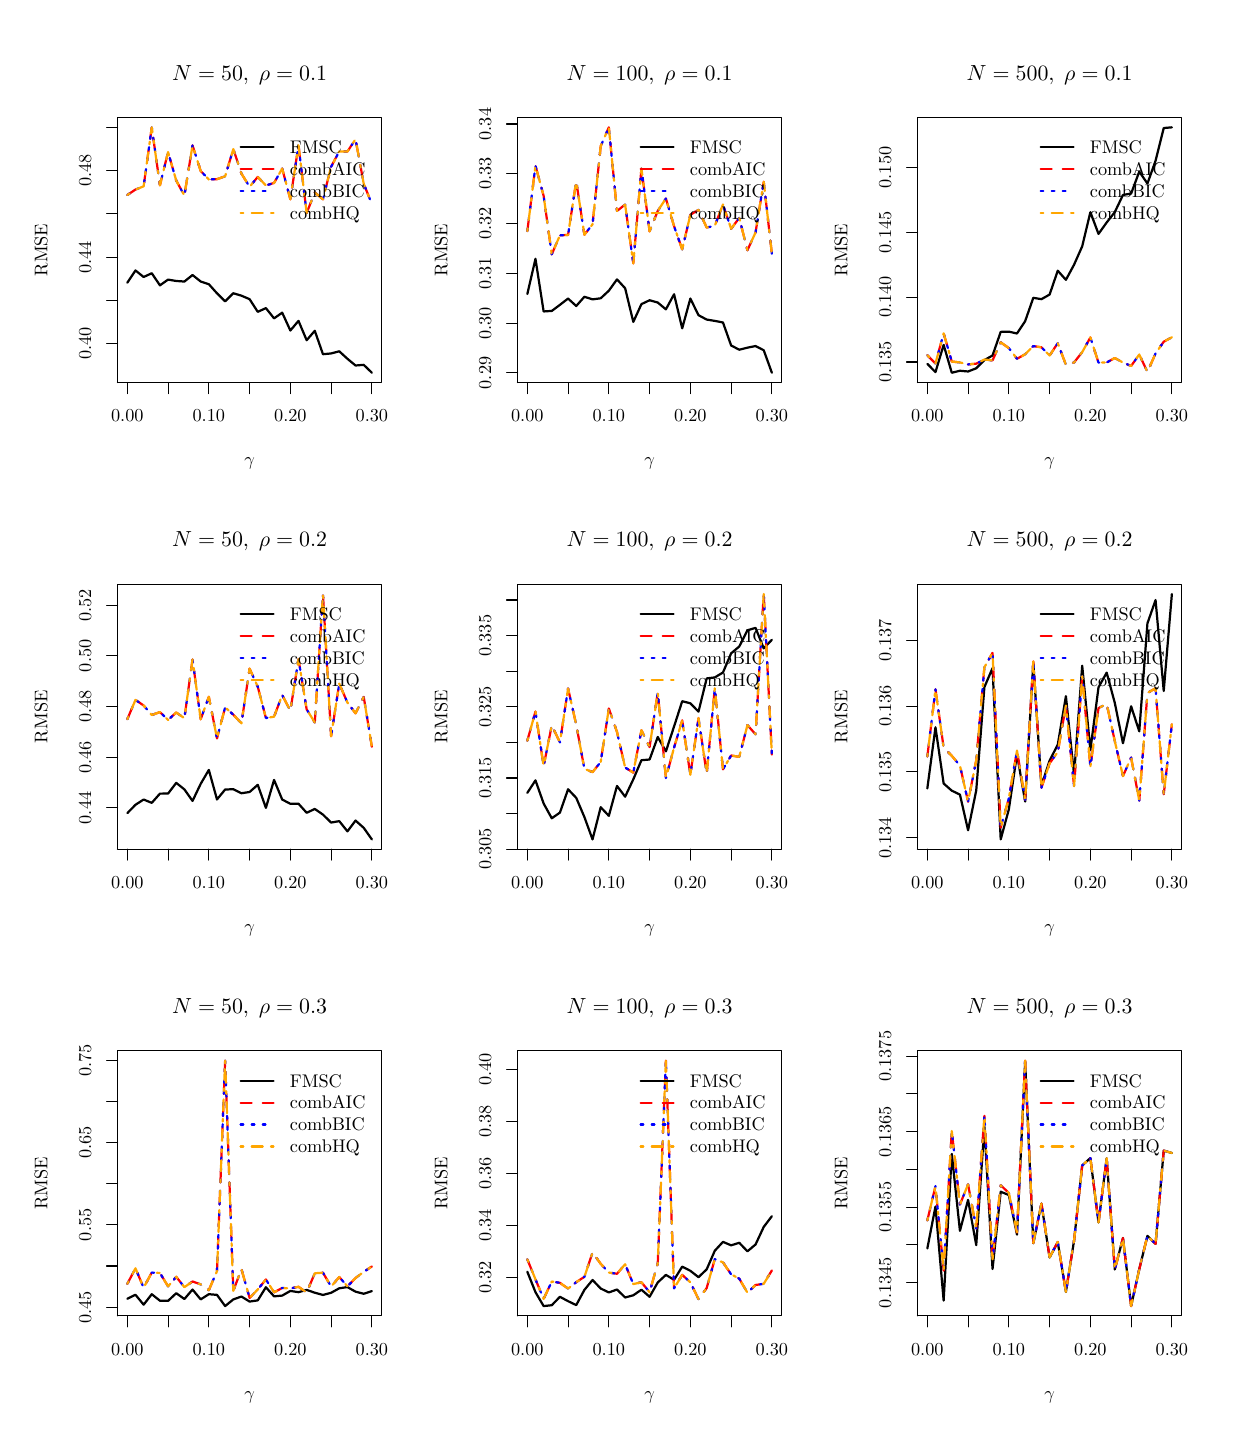
\begin{tikzpicture}[x=1pt,y=1pt]
\definecolor[named]{fillColor}{rgb}{1.00,1.00,1.00}
\path[use as bounding box,fill=fillColor,fill opacity=0.00] (0,0) rectangle (433.62,505.89);
\begin{scope}
\path[clip] ( 32.47,377.65) rectangle (127.91,473.42);
\definecolor[named]{drawColor}{rgb}{0.00,0.00,0.00}

\path[draw=drawColor,line width= 0.8pt,line join=round,line cap=round] ( 36.01,413.73) --
	( 38.95,418.16) --
	( 41.90,415.79) --
	( 44.84,417.15) --
	( 47.79,412.78) --
	( 50.73,414.85) --
	( 53.68,414.35) --
	( 56.63,414.15) --
	( 59.57,416.51) --
	( 62.52,414.16) --
	( 65.46,413.19) --
	( 68.41,409.90) --
	( 71.35,406.99) --
	( 74.30,409.92) --
	( 77.24,409.04) --
	( 80.19,407.78) --
	( 83.14,403.20) --
	( 86.08,404.55) --
	( 89.03,400.84) --
	( 91.97,402.90) --
	( 94.92,396.45) --
	( 97.86,399.94) --
	(100.81,392.95) --
	(103.75,396.35) --
	(106.70,387.89) --
	(109.65,388.17) --
	(112.59,388.94) --
	(115.54,386.24) --
	(118.48,383.81) --
	(121.43,384.05) --
	(124.37,381.20);
\end{scope}
\begin{scope}
\path[clip] (  0.00,  0.00) rectangle (433.62,505.89);
\definecolor[named]{drawColor}{rgb}{0.00,0.00,0.00}

\path[draw=drawColor,line width= 0.4pt,line join=round,line cap=round] ( 36.01,377.65) -- (124.37,377.65);

\path[draw=drawColor,line width= 0.4pt,line join=round,line cap=round] ( 36.01,377.65) -- ( 36.01,373.69);

\path[draw=drawColor,line width= 0.4pt,line join=round,line cap=round] ( 50.73,377.65) -- ( 50.73,373.69);

\path[draw=drawColor,line width= 0.4pt,line join=round,line cap=round] ( 65.46,377.65) -- ( 65.46,373.69);

\path[draw=drawColor,line width= 0.4pt,line join=round,line cap=round] ( 80.19,377.65) -- ( 80.19,373.69);

\path[draw=drawColor,line width= 0.4pt,line join=round,line cap=round] ( 94.92,377.65) -- ( 94.92,373.69);

\path[draw=drawColor,line width= 0.4pt,line join=round,line cap=round] (109.65,377.65) -- (109.65,373.69);

\path[draw=drawColor,line width= 0.4pt,line join=round,line cap=round] (124.37,377.65) -- (124.37,373.69);

\node[text=drawColor,anchor=base,inner sep=0pt, outer sep=0pt, scale=  0.66] at ( 36.01,363.40) {0.00};

\node[text=drawColor,anchor=base,inner sep=0pt, outer sep=0pt, scale=  0.66] at ( 65.46,363.40) {0.10};

\node[text=drawColor,anchor=base,inner sep=0pt, outer sep=0pt, scale=  0.66] at ( 94.92,363.40) {0.20};

\node[text=drawColor,anchor=base,inner sep=0pt, outer sep=0pt, scale=  0.66] at (124.37,363.40) {0.30};

\path[draw=drawColor,line width= 0.4pt,line join=round,line cap=round] ( 32.47,391.74) -- ( 32.47,469.81);

\path[draw=drawColor,line width= 0.4pt,line join=round,line cap=round] ( 32.47,391.74) -- ( 28.51,391.74);

\path[draw=drawColor,line width= 0.4pt,line join=round,line cap=round] ( 32.47,407.35) -- ( 28.51,407.35);

\path[draw=drawColor,line width= 0.4pt,line join=round,line cap=round] ( 32.47,422.96) -- ( 28.51,422.96);

\path[draw=drawColor,line width= 0.4pt,line join=round,line cap=round] ( 32.47,438.58) -- ( 28.51,438.58);

\path[draw=drawColor,line width= 0.4pt,line join=round,line cap=round] ( 32.47,454.19) -- ( 28.51,454.19);

\path[draw=drawColor,line width= 0.4pt,line join=round,line cap=round] ( 32.47,469.81) -- ( 28.51,469.81);

\node[text=drawColor,rotate= 90.00,anchor=base,inner sep=0pt, outer sep=0pt, scale=  0.66] at ( 22.97,391.74) {0.40};

\node[text=drawColor,rotate= 90.00,anchor=base,inner sep=0pt, outer sep=0pt, scale=  0.66] at ( 22.97,422.96) {0.44};

\node[text=drawColor,rotate= 90.00,anchor=base,inner sep=0pt, outer sep=0pt, scale=  0.66] at ( 22.97,454.19) {0.48};

\path[draw=drawColor,line width= 0.4pt,line join=round,line cap=round] ( 32.47,377.65) --
	(127.91,377.65) --
	(127.91,473.42) --
	( 32.47,473.42) --
	( 32.47,377.65);
\end{scope}
\begin{scope}
\path[clip] (  0.00,337.26) rectangle (144.54,505.89);
\definecolor[named]{drawColor}{rgb}{0.00,0.00,0.00}

\node[text=drawColor,anchor=base,inner sep=0pt, outer sep=0pt, scale=  0.79] at ( 80.19,486.92) {\bfseries $N=50, \;\rho=0.1$};

\node[text=drawColor,anchor=base,inner sep=0pt, outer sep=0pt, scale=  0.66] at ( 80.19,347.56) {$\gamma$};

\node[text=drawColor,rotate= 90.00,anchor=base,inner sep=0pt, outer sep=0pt, scale=  0.66] at (  7.13,425.53) {RMSE};
\end{scope}
\begin{scope}
\path[clip] ( 32.47,377.65) rectangle (127.91,473.42);
\definecolor[named]{drawColor}{rgb}{1.00,0.00,0.00}

\path[draw=drawColor,line width= 0.8pt,dash pattern=on 4pt off 4pt ,line join=round,line cap=round] ( 36.01,445.42) --
	( 38.95,447.38) --
	( 41.90,448.56) --
	( 44.84,469.87) --
	( 47.79,448.92) --
	( 50.73,460.94) --
	( 53.68,450.64) --
	( 56.63,445.22) --
	( 59.57,463.37) --
	( 62.52,454.09) --
	( 65.46,451.04) --
	( 68.41,451.15) --
	( 71.35,452.18) --
	( 74.30,462.01) --
	( 77.24,453.17) --
	( 80.19,448.38) --
	( 83.14,451.95) --
	( 86.08,448.87) --
	( 89.03,449.78) --
	( 91.97,454.97) --
	( 94.92,443.85) --
	( 97.86,463.38) --
	(100.81,438.92) --
	(103.75,446.33) --
	(106.70,443.87) --
	(109.65,455.64) --
	(112.59,461.17) --
	(115.54,461.13) --
	(118.48,465.58) --
	(121.43,449.47) --
	(124.37,442.13);
\definecolor[named]{drawColor}{rgb}{0.00,0.00,1.00}

\path[draw=drawColor,line width= 0.8pt,dash pattern=on 1pt off 3pt ,line join=round,line cap=round] ( 36.01,445.42) --
	( 38.95,447.38) --
	( 41.90,448.56) --
	( 44.84,469.87) --
	( 47.79,448.92) --
	( 50.73,460.94) --
	( 53.68,450.64) --
	( 56.63,445.22) --
	( 59.57,463.37) --
	( 62.52,454.09) --
	( 65.46,451.04) --
	( 68.41,451.15) --
	( 71.35,452.18) --
	( 74.30,462.01) --
	( 77.24,453.17) --
	( 80.19,448.38) --
	( 83.14,451.95) --
	( 86.08,448.87) --
	( 89.03,449.78) --
	( 91.97,454.97) --
	( 94.92,443.85) --
	( 97.86,463.38) --
	(100.81,438.92) --
	(103.75,446.33) --
	(106.70,443.87) --
	(109.65,455.64) --
	(112.59,461.17) --
	(115.54,461.13) --
	(118.48,465.58) --
	(121.43,449.47) --
	(124.37,442.13);
\definecolor[named]{drawColor}{rgb}{1.00,0.65,0.00}

\path[draw=drawColor,line width= 0.8pt,dash pattern=on 1pt off 3pt on 4pt off 3pt ,line join=round,line cap=round] ( 36.01,445.42) --
	( 38.95,447.38) --
	( 41.90,448.56) --
	( 44.84,469.87) --
	( 47.79,448.92) --
	( 50.73,460.94) --
	( 53.68,450.64) --
	( 56.63,445.22) --
	( 59.57,463.37) --
	( 62.52,454.09) --
	( 65.46,451.04) --
	( 68.41,451.15) --
	( 71.35,452.18) --
	( 74.30,462.01) --
	( 77.24,453.17) --
	( 80.19,448.38) --
	( 83.14,451.95) --
	( 86.08,448.87) --
	( 89.03,449.78) --
	( 91.97,454.97) --
	( 94.92,443.85) --
	( 97.86,463.38) --
	(100.81,438.92) --
	(103.75,446.33) --
	(106.70,443.87) --
	(109.65,455.64) --
	(112.59,461.17) --
	(115.54,461.13) --
	(118.48,465.58) --
	(121.43,449.47) --
	(124.37,442.13);
\definecolor[named]{drawColor}{rgb}{0.00,0.00,0.00}

\path[draw=drawColor,line width= 0.8pt,line join=round,line cap=round] ( 76.94,462.63) -- ( 88.82,462.63);
\definecolor[named]{drawColor}{rgb}{1.00,0.00,0.00}

\path[draw=drawColor,line width= 0.8pt,dash pattern=on 4pt off 4pt ,line join=round,line cap=round] ( 76.94,454.71) -- ( 88.82,454.71);
\definecolor[named]{drawColor}{rgb}{0.00,0.00,1.00}

\path[draw=drawColor,line width= 0.8pt,dash pattern=on 1pt off 3pt ,line join=round,line cap=round] ( 76.94,446.79) -- ( 88.82,446.79);
\definecolor[named]{drawColor}{rgb}{1.00,0.65,0.00}

\path[draw=drawColor,line width= 0.8pt,dash pattern=on 1pt off 3pt on 4pt off 3pt ,line join=round,line cap=round] ( 76.94,438.87) -- ( 88.82,438.87);
\definecolor[named]{drawColor}{rgb}{0.00,0.00,0.00}

\node[text=drawColor,anchor=base west,inner sep=0pt, outer sep=0pt, scale=  0.66] at ( 94.76,460.35) {FMSC};

\node[text=drawColor,anchor=base west,inner sep=0pt, outer sep=0pt, scale=  0.66] at ( 94.76,452.43) {combAIC};

\node[text=drawColor,anchor=base west,inner sep=0pt, outer sep=0pt, scale=  0.66] at ( 94.76,444.51) {combBIC};

\node[text=drawColor,anchor=base west,inner sep=0pt, outer sep=0pt, scale=  0.66] at ( 94.76,436.59) {combHQ};
\end{scope}
\begin{scope}
\path[clip] (177.01,377.65) rectangle (272.45,473.42);
\definecolor[named]{drawColor}{rgb}{0.00,0.00,0.00}

\path[draw=drawColor,line width= 0.8pt,line join=round,line cap=round] (180.55,409.64) --
	(183.49,422.36) --
	(186.44,403.34) --
	(189.38,403.53) --
	(192.33,405.74) --
	(195.27,408.00) --
	(198.22,405.31) --
	(201.17,408.65) --
	(204.11,407.71) --
	(207.06,408.10) --
	(210.00,410.84) --
	(212.95,414.93) --
	(215.89,411.73) --
	(218.84,399.56) --
	(221.78,405.99) --
	(224.73,407.39) --
	(227.68,406.56) --
	(230.62,404.11) --
	(233.57,409.56) --
	(236.51,397.24) --
	(239.46,408.00) --
	(242.40,401.99) --
	(245.35,400.41) --
	(248.29,399.93) --
	(251.24,399.36) --
	(254.19,391.05) --
	(257.13,389.51) --
	(260.08,390.25) --
	(263.02,390.84) --
	(265.97,389.32) --
	(268.91,381.20);
\end{scope}
\begin{scope}
\path[clip] (  0.00,  0.00) rectangle (433.62,505.89);
\definecolor[named]{drawColor}{rgb}{0.00,0.00,0.00}

\path[draw=drawColor,line width= 0.4pt,line join=round,line cap=round] (180.55,377.65) -- (268.91,377.65);

\path[draw=drawColor,line width= 0.4pt,line join=round,line cap=round] (180.55,377.65) -- (180.55,373.69);

\path[draw=drawColor,line width= 0.4pt,line join=round,line cap=round] (195.27,377.65) -- (195.27,373.69);

\path[draw=drawColor,line width= 0.4pt,line join=round,line cap=round] (210.00,377.65) -- (210.00,373.69);

\path[draw=drawColor,line width= 0.4pt,line join=round,line cap=round] (224.73,377.65) -- (224.73,373.69);

\path[draw=drawColor,line width= 0.4pt,line join=round,line cap=round] (239.46,377.65) -- (239.46,373.69);

\path[draw=drawColor,line width= 0.4pt,line join=round,line cap=round] (254.19,377.65) -- (254.19,373.69);

\path[draw=drawColor,line width= 0.4pt,line join=round,line cap=round] (268.91,377.65) -- (268.91,373.69);

\node[text=drawColor,anchor=base,inner sep=0pt, outer sep=0pt, scale=  0.66] at (180.55,363.40) {0.00};

\node[text=drawColor,anchor=base,inner sep=0pt, outer sep=0pt, scale=  0.66] at (210.00,363.40) {0.10};

\node[text=drawColor,anchor=base,inner sep=0pt, outer sep=0pt, scale=  0.66] at (239.46,363.40) {0.20};

\node[text=drawColor,anchor=base,inner sep=0pt, outer sep=0pt, scale=  0.66] at (268.91,363.40) {0.30};

\path[draw=drawColor,line width= 0.4pt,line join=round,line cap=round] (177.01,381.13) -- (177.01,471.09);

\path[draw=drawColor,line width= 0.4pt,line join=round,line cap=round] (177.01,381.13) -- (173.05,381.13);

\path[draw=drawColor,line width= 0.4pt,line join=round,line cap=round] (177.01,399.12) -- (173.05,399.12);

\path[draw=drawColor,line width= 0.4pt,line join=round,line cap=round] (177.01,417.11) -- (173.05,417.11);

\path[draw=drawColor,line width= 0.4pt,line join=round,line cap=round] (177.01,435.10) -- (173.05,435.10);

\path[draw=drawColor,line width= 0.4pt,line join=round,line cap=round] (177.01,453.10) -- (173.05,453.10);

\path[draw=drawColor,line width= 0.4pt,line join=round,line cap=round] (177.01,471.09) -- (173.05,471.09);

\node[text=drawColor,rotate= 90.00,anchor=base,inner sep=0pt, outer sep=0pt, scale=  0.66] at (167.51,381.13) {0.29};

\node[text=drawColor,rotate= 90.00,anchor=base,inner sep=0pt, outer sep=0pt, scale=  0.66] at (167.51,399.12) {0.30};

\node[text=drawColor,rotate= 90.00,anchor=base,inner sep=0pt, outer sep=0pt, scale=  0.66] at (167.51,417.11) {0.31};

\node[text=drawColor,rotate= 90.00,anchor=base,inner sep=0pt, outer sep=0pt, scale=  0.66] at (167.51,435.10) {0.32};

\node[text=drawColor,rotate= 90.00,anchor=base,inner sep=0pt, outer sep=0pt, scale=  0.66] at (167.51,453.10) {0.33};

\node[text=drawColor,rotate= 90.00,anchor=base,inner sep=0pt, outer sep=0pt, scale=  0.66] at (167.51,471.09) {0.34};

\path[draw=drawColor,line width= 0.4pt,line join=round,line cap=round] (177.01,377.65) --
	(272.45,377.65) --
	(272.45,473.42) --
	(177.01,473.42) --
	(177.01,377.65);
\end{scope}
\begin{scope}
\path[clip] (144.54,337.26) rectangle (289.08,505.89);
\definecolor[named]{drawColor}{rgb}{0.00,0.00,0.00}

\node[text=drawColor,anchor=base,inner sep=0pt, outer sep=0pt, scale=  0.79] at (224.73,486.92) {\bfseries $N=100, \;\rho=0.1$};

\node[text=drawColor,anchor=base,inner sep=0pt, outer sep=0pt, scale=  0.66] at (224.73,347.56) {$\gamma$};

\node[text=drawColor,rotate= 90.00,anchor=base,inner sep=0pt, outer sep=0pt, scale=  0.66] at (151.67,425.53) {RMSE};
\end{scope}
\begin{scope}
\path[clip] (177.01,377.65) rectangle (272.45,473.42);
\definecolor[named]{drawColor}{rgb}{1.00,0.00,0.00}

\path[draw=drawColor,line width= 0.8pt,dash pattern=on 4pt off 4pt ,line join=round,line cap=round] (180.55,432.38) --
	(183.49,456.00) --
	(186.44,445.11) --
	(189.38,424.00) --
	(192.33,430.84) --
	(195.27,430.99) --
	(198.22,450.41) --
	(201.17,431.06) --
	(204.11,434.82) --
	(207.06,463.04) --
	(210.00,469.87) --
	(212.95,439.66) --
	(215.89,441.97) --
	(218.84,420.70) --
	(221.78,455.03) --
	(224.73,432.27) --
	(227.68,439.68) --
	(230.62,444.15) --
	(233.57,434.15) --
	(236.51,425.74) --
	(239.46,438.28) --
	(242.40,440.03) --
	(245.35,433.68) --
	(248.29,434.30) --
	(251.24,441.99) --
	(254.19,433.21) --
	(257.13,437.16) --
	(260.08,425.45) --
	(263.02,431.90) --
	(265.97,450.18) --
	(268.91,424.19);
\definecolor[named]{drawColor}{rgb}{0.00,0.00,1.00}

\path[draw=drawColor,line width= 0.8pt,dash pattern=on 1pt off 3pt ,line join=round,line cap=round] (180.55,432.38) --
	(183.49,456.00) --
	(186.44,445.11) --
	(189.38,424.00) --
	(192.33,430.84) --
	(195.27,430.99) --
	(198.22,450.41) --
	(201.17,431.06) --
	(204.11,434.82) --
	(207.06,463.04) --
	(210.00,469.87) --
	(212.95,439.66) --
	(215.89,441.97) --
	(218.84,420.70) --
	(221.78,455.03) --
	(224.73,432.27) --
	(227.68,439.68) --
	(230.62,444.15) --
	(233.57,434.15) --
	(236.51,425.74) --
	(239.46,438.28) --
	(242.40,440.03) --
	(245.35,433.68) --
	(248.29,434.30) --
	(251.24,441.99) --
	(254.19,433.21) --
	(257.13,437.16) --
	(260.08,425.45) --
	(263.02,431.90) --
	(265.97,450.18) --
	(268.91,424.19);
\definecolor[named]{drawColor}{rgb}{1.00,0.65,0.00}

\path[draw=drawColor,line width= 0.8pt,dash pattern=on 1pt off 3pt on 4pt off 3pt ,line join=round,line cap=round] (180.55,432.38) --
	(183.49,456.00) --
	(186.44,445.11) --
	(189.38,424.00) --
	(192.33,430.84) --
	(195.27,430.99) --
	(198.22,450.41) --
	(201.17,431.06) --
	(204.11,434.82) --
	(207.06,463.04) --
	(210.00,469.87) --
	(212.95,439.66) --
	(215.89,441.97) --
	(218.84,420.70) --
	(221.78,455.03) --
	(224.73,432.27) --
	(227.68,439.68) --
	(230.62,444.15) --
	(233.57,434.15) --
	(236.51,425.74) --
	(239.46,438.28) --
	(242.40,440.03) --
	(245.35,433.68) --
	(248.29,434.30) --
	(251.24,441.99) --
	(254.19,433.21) --
	(257.13,437.16) --
	(260.08,425.45) --
	(263.02,431.90) --
	(265.97,450.18) --
	(268.91,424.19);
\definecolor[named]{drawColor}{rgb}{0.00,0.00,0.00}

\path[draw=drawColor,line width= 0.8pt,line join=round,line cap=round] (221.48,462.63) -- (233.36,462.63);
\definecolor[named]{drawColor}{rgb}{1.00,0.00,0.00}

\path[draw=drawColor,line width= 0.8pt,dash pattern=on 4pt off 4pt ,line join=round,line cap=round] (221.48,454.71) -- (233.36,454.71);
\definecolor[named]{drawColor}{rgb}{0.00,0.00,1.00}

\path[draw=drawColor,line width= 0.8pt,dash pattern=on 1pt off 3pt ,line join=round,line cap=round] (221.48,446.79) -- (233.36,446.79);
\definecolor[named]{drawColor}{rgb}{1.00,0.65,0.00}

\path[draw=drawColor,line width= 0.8pt,dash pattern=on 1pt off 3pt on 4pt off 3pt ,line join=round,line cap=round] (221.48,438.87) -- (233.36,438.87);
\definecolor[named]{drawColor}{rgb}{0.00,0.00,0.00}

\node[text=drawColor,anchor=base west,inner sep=0pt, outer sep=0pt, scale=  0.66] at (239.30,460.35) {FMSC};

\node[text=drawColor,anchor=base west,inner sep=0pt, outer sep=0pt, scale=  0.66] at (239.30,452.43) {combAIC};

\node[text=drawColor,anchor=base west,inner sep=0pt, outer sep=0pt, scale=  0.66] at (239.30,444.51) {combBIC};

\node[text=drawColor,anchor=base west,inner sep=0pt, outer sep=0pt, scale=  0.66] at (239.30,436.59) {combHQ};
\end{scope}
\begin{scope}
\path[clip] (321.55,377.65) rectangle (416.99,473.42);
\definecolor[named]{drawColor}{rgb}{0.00,0.00,0.00}

\path[draw=drawColor,line width= 0.8pt,line join=round,line cap=round] (325.09,384.42) --
	(328.03,381.41) --
	(330.98,391.26) --
	(333.92,381.20) --
	(336.87,381.91) --
	(339.81,381.65) --
	(342.76,382.80) --
	(345.71,385.77) --
	(348.65,387.43) --
	(351.60,395.96) --
	(354.54,396.04) --
	(357.49,395.38) --
	(360.43,399.82) --
	(363.38,408.27) --
	(366.32,407.77) --
	(369.27,409.45) --
	(372.22,418.07) --
	(375.16,414.76) --
	(378.11,420.24) --
	(381.05,426.88) --
	(384.00,439.21) --
	(386.94,431.36) --
	(389.89,435.49) --
	(392.83,439.25) --
	(395.78,445.44) --
	(398.73,445.94) --
	(401.67,453.87) --
	(404.62,449.56) --
	(407.56,457.81) --
	(410.51,469.62) --
	(413.45,469.87);
\end{scope}
\begin{scope}
\path[clip] (  0.00,  0.00) rectangle (433.62,505.89);
\definecolor[named]{drawColor}{rgb}{0.00,0.00,0.00}

\path[draw=drawColor,line width= 0.4pt,line join=round,line cap=round] (325.09,377.65) -- (413.45,377.65);

\path[draw=drawColor,line width= 0.4pt,line join=round,line cap=round] (325.09,377.65) -- (325.09,373.69);

\path[draw=drawColor,line width= 0.4pt,line join=round,line cap=round] (339.81,377.65) -- (339.81,373.69);

\path[draw=drawColor,line width= 0.4pt,line join=round,line cap=round] (354.54,377.65) -- (354.54,373.69);

\path[draw=drawColor,line width= 0.4pt,line join=round,line cap=round] (369.27,377.65) -- (369.27,373.69);

\path[draw=drawColor,line width= 0.4pt,line join=round,line cap=round] (384.00,377.65) -- (384.00,373.69);

\path[draw=drawColor,line width= 0.4pt,line join=round,line cap=round] (398.73,377.65) -- (398.73,373.69);

\path[draw=drawColor,line width= 0.4pt,line join=round,line cap=round] (413.45,377.65) -- (413.45,373.69);

\node[text=drawColor,anchor=base,inner sep=0pt, outer sep=0pt, scale=  0.66] at (325.09,363.40) {0.00};

\node[text=drawColor,anchor=base,inner sep=0pt, outer sep=0pt, scale=  0.66] at (354.54,363.40) {0.10};

\node[text=drawColor,anchor=base,inner sep=0pt, outer sep=0pt, scale=  0.66] at (384.00,363.40) {0.20};

\node[text=drawColor,anchor=base,inner sep=0pt, outer sep=0pt, scale=  0.66] at (413.45,363.40) {0.30};

\path[draw=drawColor,line width= 0.4pt,line join=round,line cap=round] (321.55,385.08) -- (321.55,455.36);

\path[draw=drawColor,line width= 0.4pt,line join=round,line cap=round] (321.55,385.08) -- (317.59,385.08);

\path[draw=drawColor,line width= 0.4pt,line join=round,line cap=round] (321.55,408.51) -- (317.59,408.51);

\path[draw=drawColor,line width= 0.4pt,line join=round,line cap=round] (321.55,431.93) -- (317.59,431.93);

\path[draw=drawColor,line width= 0.4pt,line join=round,line cap=round] (321.55,455.36) -- (317.59,455.36);

\node[text=drawColor,rotate= 90.00,anchor=base,inner sep=0pt, outer sep=0pt, scale=  0.66] at (312.05,385.08) {0.135};

\node[text=drawColor,rotate= 90.00,anchor=base,inner sep=0pt, outer sep=0pt, scale=  0.66] at (312.05,408.51) {0.140};

\node[text=drawColor,rotate= 90.00,anchor=base,inner sep=0pt, outer sep=0pt, scale=  0.66] at (312.05,431.93) {0.145};

\node[text=drawColor,rotate= 90.00,anchor=base,inner sep=0pt, outer sep=0pt, scale=  0.66] at (312.05,455.36) {0.150};

\path[draw=drawColor,line width= 0.4pt,line join=round,line cap=round] (321.55,377.65) --
	(416.99,377.65) --
	(416.99,473.42) --
	(321.55,473.42) --
	(321.55,377.65);
\end{scope}
\begin{scope}
\path[clip] (289.08,337.26) rectangle (433.62,505.89);
\definecolor[named]{drawColor}{rgb}{0.00,0.00,0.00}

\node[text=drawColor,anchor=base,inner sep=0pt, outer sep=0pt, scale=  0.79] at (369.27,486.92) {\bfseries $N=500, \;\rho=0.1$};

\node[text=drawColor,anchor=base,inner sep=0pt, outer sep=0pt, scale=  0.66] at (369.27,347.56) {$\gamma$};

\node[text=drawColor,rotate= 90.00,anchor=base,inner sep=0pt, outer sep=0pt, scale=  0.66] at (296.21,425.53) {RMSE};
\end{scope}
\begin{scope}
\path[clip] (321.55,377.65) rectangle (416.99,473.42);
\definecolor[named]{drawColor}{rgb}{1.00,0.00,0.00}

\path[draw=drawColor,line width= 0.8pt,dash pattern=on 4pt off 4pt ,line join=round,line cap=round] (325.09,387.51) --
	(328.03,384.54) --
	(330.98,395.44) --
	(333.92,385.25) --
	(336.87,384.91) --
	(339.81,384.20) --
	(342.76,384.48) --
	(345.71,385.97) --
	(348.65,385.67) --
	(351.60,392.19) --
	(354.54,390.09) --
	(357.49,386.25) --
	(360.43,387.86) --
	(363.38,390.82) --
	(366.32,390.38) --
	(369.27,387.41) --
	(372.22,391.89) --
	(375.16,384.06) --
	(378.11,384.92) --
	(381.05,388.65) --
	(384.00,393.94) --
	(386.94,384.85) --
	(389.89,384.89) --
	(392.83,386.52) --
	(395.78,384.89) --
	(398.73,383.64) --
	(401.67,387.79) --
	(404.62,381.47) --
	(407.56,388.17) --
	(410.51,392.41) --
	(413.45,394.01);
\definecolor[named]{drawColor}{rgb}{0.00,0.00,1.00}

\path[draw=drawColor,line width= 0.8pt,dash pattern=on 1pt off 3pt ,line join=round,line cap=round] (325.09,387.51) --
	(328.03,384.54) --
	(330.98,395.44) --
	(333.92,385.25) --
	(336.87,384.91) --
	(339.81,384.20) --
	(342.76,384.48) --
	(345.71,385.97) --
	(348.65,385.67) --
	(351.60,392.19) --
	(354.54,390.09) --
	(357.49,386.25) --
	(360.43,387.86) --
	(363.38,390.82) --
	(366.32,390.38) --
	(369.27,387.41) --
	(372.22,391.89) --
	(375.16,384.06) --
	(378.11,384.92) --
	(381.05,388.65) --
	(384.00,393.94) --
	(386.94,384.85) --
	(389.89,384.89) --
	(392.83,386.52) --
	(395.78,384.89) --
	(398.73,383.64) --
	(401.67,387.79) --
	(404.62,381.47) --
	(407.56,388.17) --
	(410.51,392.41) --
	(413.45,394.01);
\definecolor[named]{drawColor}{rgb}{1.00,0.65,0.00}

\path[draw=drawColor,line width= 0.8pt,dash pattern=on 1pt off 3pt on 4pt off 3pt ,line join=round,line cap=round] (325.09,387.51) --
	(328.03,384.54) --
	(330.98,395.44) --
	(333.92,385.25) --
	(336.87,384.91) --
	(339.81,384.20) --
	(342.76,384.48) --
	(345.71,385.97) --
	(348.65,385.67) --
	(351.60,392.19) --
	(354.54,390.09) --
	(357.49,386.25) --
	(360.43,387.86) --
	(363.38,390.82) --
	(366.32,390.38) --
	(369.27,387.41) --
	(372.22,391.89) --
	(375.16,384.06) --
	(378.11,384.92) --
	(381.05,388.65) --
	(384.00,393.94) --
	(386.94,384.85) --
	(389.89,384.89) --
	(392.83,386.52) --
	(395.78,384.89) --
	(398.73,383.64) --
	(401.67,387.79) --
	(404.62,381.47) --
	(407.56,388.17) --
	(410.51,392.41) --
	(413.45,394.01);
\definecolor[named]{drawColor}{rgb}{0.00,0.00,0.00}

\path[draw=drawColor,line width= 0.8pt,line join=round,line cap=round] (366.02,462.63) -- (377.90,462.63);
\definecolor[named]{drawColor}{rgb}{1.00,0.00,0.00}

\path[draw=drawColor,line width= 0.8pt,dash pattern=on 4pt off 4pt ,line join=round,line cap=round] (366.02,454.71) -- (377.90,454.71);
\definecolor[named]{drawColor}{rgb}{0.00,0.00,1.00}

\path[draw=drawColor,line width= 0.8pt,dash pattern=on 1pt off 3pt ,line join=round,line cap=round] (366.02,446.79) -- (377.90,446.79);
\definecolor[named]{drawColor}{rgb}{1.00,0.65,0.00}

\path[draw=drawColor,line width= 0.8pt,dash pattern=on 1pt off 3pt on 4pt off 3pt ,line join=round,line cap=round] (366.02,438.87) -- (377.90,438.87);
\definecolor[named]{drawColor}{rgb}{0.00,0.00,0.00}

\node[text=drawColor,anchor=base west,inner sep=0pt, outer sep=0pt, scale=  0.66] at (383.84,460.35) {FMSC};

\node[text=drawColor,anchor=base west,inner sep=0pt, outer sep=0pt, scale=  0.66] at (383.84,452.43) {combAIC};

\node[text=drawColor,anchor=base west,inner sep=0pt, outer sep=0pt, scale=  0.66] at (383.84,444.51) {combBIC};

\node[text=drawColor,anchor=base west,inner sep=0pt, outer sep=0pt, scale=  0.66] at (383.84,436.59) {combHQ};
\end{scope}
\begin{scope}
\path[clip] ( 32.47,209.02) rectangle (127.91,304.79);
\definecolor[named]{drawColor}{rgb}{0.00,0.00,0.00}

\path[draw=drawColor,line width= 0.8pt,line join=round,line cap=round] ( 36.01,222.06) --
	( 38.95,225.07) --
	( 41.90,226.98) --
	( 44.84,225.77) --
	( 47.79,229.11) --
	( 50.73,229.13) --
	( 53.68,233.00) --
	( 56.63,230.64) --
	( 59.57,226.47) --
	( 62.52,232.65) --
	( 65.46,237.68) --
	( 68.41,227.01) --
	( 71.35,230.59) --
	( 74.30,230.71) --
	( 77.24,229.25) --
	( 80.19,229.70) --
	( 83.14,232.29) --
	( 86.08,223.96) --
	( 89.03,234.06) --
	( 91.97,226.98) --
	( 94.92,225.43) --
	( 97.86,225.46) --
	(100.81,222.19) --
	(103.75,223.57) --
	(106.70,221.53) --
	(109.65,218.65) --
	(112.59,219.18) --
	(115.54,215.47) --
	(118.48,219.37) --
	(121.43,216.75) --
	(124.37,212.57);
\end{scope}
\begin{scope}
\path[clip] (  0.00,  0.00) rectangle (433.62,505.89);
\definecolor[named]{drawColor}{rgb}{0.00,0.00,0.00}

\path[draw=drawColor,line width= 0.4pt,line join=round,line cap=round] ( 36.01,209.02) -- (124.37,209.02);

\path[draw=drawColor,line width= 0.4pt,line join=round,line cap=round] ( 36.01,209.02) -- ( 36.01,205.06);

\path[draw=drawColor,line width= 0.4pt,line join=round,line cap=round] ( 50.73,209.02) -- ( 50.73,205.06);

\path[draw=drawColor,line width= 0.4pt,line join=round,line cap=round] ( 65.46,209.02) -- ( 65.46,205.06);

\path[draw=drawColor,line width= 0.4pt,line join=round,line cap=round] ( 80.19,209.02) -- ( 80.19,205.06);

\path[draw=drawColor,line width= 0.4pt,line join=round,line cap=round] ( 94.92,209.02) -- ( 94.92,205.06);

\path[draw=drawColor,line width= 0.4pt,line join=round,line cap=round] (109.65,209.02) -- (109.65,205.06);

\path[draw=drawColor,line width= 0.4pt,line join=round,line cap=round] (124.37,209.02) -- (124.37,205.06);

\node[text=drawColor,anchor=base,inner sep=0pt, outer sep=0pt, scale=  0.66] at ( 36.01,194.77) {0.00};

\node[text=drawColor,anchor=base,inner sep=0pt, outer sep=0pt, scale=  0.66] at ( 65.46,194.77) {0.10};

\node[text=drawColor,anchor=base,inner sep=0pt, outer sep=0pt, scale=  0.66] at ( 94.92,194.77) {0.20};

\node[text=drawColor,anchor=base,inner sep=0pt, outer sep=0pt, scale=  0.66] at (124.37,194.77) {0.30};

\path[draw=drawColor,line width= 0.4pt,line join=round,line cap=round] ( 32.47,223.95) -- ( 32.47,297.21);

\path[draw=drawColor,line width= 0.4pt,line join=round,line cap=round] ( 32.47,223.95) -- ( 28.51,223.95);

\path[draw=drawColor,line width= 0.4pt,line join=round,line cap=round] ( 32.47,242.27) -- ( 28.51,242.27);

\path[draw=drawColor,line width= 0.4pt,line join=round,line cap=round] ( 32.47,260.58) -- ( 28.51,260.58);

\path[draw=drawColor,line width= 0.4pt,line join=round,line cap=round] ( 32.47,278.90) -- ( 28.51,278.90);

\path[draw=drawColor,line width= 0.4pt,line join=round,line cap=round] ( 32.47,297.21) -- ( 28.51,297.21);

\node[text=drawColor,rotate= 90.00,anchor=base,inner sep=0pt, outer sep=0pt, scale=  0.66] at ( 22.97,223.95) {0.44};

\node[text=drawColor,rotate= 90.00,anchor=base,inner sep=0pt, outer sep=0pt, scale=  0.66] at ( 22.97,242.27) {0.46};

\node[text=drawColor,rotate= 90.00,anchor=base,inner sep=0pt, outer sep=0pt, scale=  0.66] at ( 22.97,260.58) {0.48};

\node[text=drawColor,rotate= 90.00,anchor=base,inner sep=0pt, outer sep=0pt, scale=  0.66] at ( 22.97,278.90) {0.50};

\node[text=drawColor,rotate= 90.00,anchor=base,inner sep=0pt, outer sep=0pt, scale=  0.66] at ( 22.97,297.21) {0.52};

\path[draw=drawColor,line width= 0.4pt,line join=round,line cap=round] ( 32.47,209.02) --
	(127.91,209.02) --
	(127.91,304.79) --
	( 32.47,304.79) --
	( 32.47,209.02);
\end{scope}
\begin{scope}
\path[clip] (  0.00,168.63) rectangle (144.54,337.26);
\definecolor[named]{drawColor}{rgb}{0.00,0.00,0.00}

\node[text=drawColor,anchor=base,inner sep=0pt, outer sep=0pt, scale=  0.79] at ( 80.19,318.29) {\bfseries $N=50, \;\rho=0.2$};

\node[text=drawColor,anchor=base,inner sep=0pt, outer sep=0pt, scale=  0.66] at ( 80.19,178.93) {$\gamma$};

\node[text=drawColor,rotate= 90.00,anchor=base,inner sep=0pt, outer sep=0pt, scale=  0.66] at (  7.13,256.90) {RMSE};
\end{scope}
\begin{scope}
\path[clip] ( 32.47,209.02) rectangle (127.91,304.79);
\definecolor[named]{drawColor}{rgb}{1.00,0.00,0.00}

\path[draw=drawColor,line width= 0.8pt,dash pattern=on 4pt off 4pt ,line join=round,line cap=round] ( 36.01,256.01) --
	( 38.95,262.97) --
	( 41.90,260.97) --
	( 44.84,257.51) --
	( 47.79,258.59) --
	( 50.73,255.73) --
	( 53.68,258.42) --
	( 56.63,256.36) --
	( 59.57,277.59) --
	( 62.52,255.98) --
	( 65.46,264.10) --
	( 68.41,249.05) --
	( 71.35,260.28) --
	( 74.30,257.64) --
	( 77.24,254.50) --
	( 80.19,274.27) --
	( 83.14,267.74) --
	( 86.08,256.43) --
	( 89.03,256.91) --
	( 91.97,264.73) --
	( 94.92,259.07) --
	( 97.86,277.72) --
	(100.81,259.54) --
	(103.75,254.84) --
	(106.70,301.24) --
	(109.65,249.85) --
	(112.59,268.86) --
	(115.54,262.01) --
	(118.48,258.13) --
	(121.43,264.08) --
	(124.37,246.05);
\definecolor[named]{drawColor}{rgb}{0.00,0.00,1.00}

\path[draw=drawColor,line width= 0.8pt,dash pattern=on 1pt off 3pt ,line join=round,line cap=round] ( 36.01,256.01) --
	( 38.95,262.97) --
	( 41.90,260.97) --
	( 44.84,257.51) --
	( 47.79,258.59) --
	( 50.73,255.73) --
	( 53.68,258.42) --
	( 56.63,256.36) --
	( 59.57,277.59) --
	( 62.52,255.98) --
	( 65.46,264.10) --
	( 68.41,249.05) --
	( 71.35,260.28) --
	( 74.30,257.64) --
	( 77.24,254.50) --
	( 80.19,274.27) --
	( 83.14,267.74) --
	( 86.08,256.43) --
	( 89.03,256.91) --
	( 91.97,264.73) --
	( 94.92,259.07) --
	( 97.86,277.72) --
	(100.81,259.54) --
	(103.75,254.84) --
	(106.70,301.24) --
	(109.65,249.85) --
	(112.59,268.86) --
	(115.54,262.01) --
	(118.48,258.13) --
	(121.43,264.08) --
	(124.37,246.05);
\definecolor[named]{drawColor}{rgb}{1.00,0.65,0.00}

\path[draw=drawColor,line width= 0.8pt,dash pattern=on 1pt off 3pt on 4pt off 3pt ,line join=round,line cap=round] ( 36.01,256.01) --
	( 38.95,262.97) --
	( 41.90,260.97) --
	( 44.84,257.51) --
	( 47.79,258.59) --
	( 50.73,255.73) --
	( 53.68,258.42) --
	( 56.63,256.36) --
	( 59.57,277.59) --
	( 62.52,255.98) --
	( 65.46,264.10) --
	( 68.41,249.05) --
	( 71.35,260.28) --
	( 74.30,257.64) --
	( 77.24,254.50) --
	( 80.19,274.27) --
	( 83.14,267.74) --
	( 86.08,256.43) --
	( 89.03,256.91) --
	( 91.97,264.73) --
	( 94.92,259.07) --
	( 97.86,277.72) --
	(100.81,259.54) --
	(103.75,254.84) --
	(106.70,301.24) --
	(109.65,249.85) --
	(112.59,268.86) --
	(115.54,262.01) --
	(118.48,258.13) --
	(121.43,264.08) --
	(124.37,246.05);
\definecolor[named]{drawColor}{rgb}{0.00,0.00,0.00}

\path[draw=drawColor,line width= 0.8pt,line join=round,line cap=round] ( 76.94,294.00) -- ( 88.82,294.00);
\definecolor[named]{drawColor}{rgb}{1.00,0.00,0.00}

\path[draw=drawColor,line width= 0.8pt,dash pattern=on 4pt off 4pt ,line join=round,line cap=round] ( 76.94,286.08) -- ( 88.82,286.08);
\definecolor[named]{drawColor}{rgb}{0.00,0.00,1.00}

\path[draw=drawColor,line width= 0.8pt,dash pattern=on 1pt off 3pt ,line join=round,line cap=round] ( 76.94,278.16) -- ( 88.82,278.16);
\definecolor[named]{drawColor}{rgb}{1.00,0.65,0.00}

\path[draw=drawColor,line width= 0.8pt,dash pattern=on 1pt off 3pt on 4pt off 3pt ,line join=round,line cap=round] ( 76.94,270.24) -- ( 88.82,270.24);
\definecolor[named]{drawColor}{rgb}{0.00,0.00,0.00}

\node[text=drawColor,anchor=base west,inner sep=0pt, outer sep=0pt, scale=  0.66] at ( 94.76,291.72) {FMSC};

\node[text=drawColor,anchor=base west,inner sep=0pt, outer sep=0pt, scale=  0.66] at ( 94.76,283.80) {combAIC};

\node[text=drawColor,anchor=base west,inner sep=0pt, outer sep=0pt, scale=  0.66] at ( 94.76,275.88) {combBIC};

\node[text=drawColor,anchor=base west,inner sep=0pt, outer sep=0pt, scale=  0.66] at ( 94.76,267.96) {combHQ};
\end{scope}
\begin{scope}
\path[clip] (177.01,209.02) rectangle (272.45,304.79);
\definecolor[named]{drawColor}{rgb}{0.00,0.00,0.00}

\path[draw=drawColor,line width= 0.8pt,line join=round,line cap=round] (180.55,229.38) --
	(183.49,233.91) --
	(186.44,225.54) --
	(189.38,220.20) --
	(192.33,222.26) --
	(195.27,230.68) --
	(198.22,227.58) --
	(201.17,220.65) --
	(204.11,212.57) --
	(207.06,224.20) --
	(210.00,221.09) --
	(212.95,231.88) --
	(215.89,228.00) --
	(218.84,234.27) --
	(221.78,241.18) --
	(224.73,241.44) --
	(227.68,249.57) --
	(230.62,244.37) --
	(233.57,253.37) --
	(236.51,262.49) --
	(239.46,261.75) --
	(242.40,258.73) --
	(245.35,270.74) --
	(248.29,271.10) --
	(251.24,272.88) --
	(254.19,279.80) --
	(257.13,282.28) --
	(260.08,288.14) --
	(263.02,289.00) --
	(265.97,281.59) --
	(268.91,284.70);
\end{scope}
\begin{scope}
\path[clip] (  0.00,  0.00) rectangle (433.62,505.89);
\definecolor[named]{drawColor}{rgb}{0.00,0.00,0.00}

\path[draw=drawColor,line width= 0.4pt,line join=round,line cap=round] (180.55,209.02) -- (268.91,209.02);

\path[draw=drawColor,line width= 0.4pt,line join=round,line cap=round] (180.55,209.02) -- (180.55,205.06);

\path[draw=drawColor,line width= 0.4pt,line join=round,line cap=round] (195.27,209.02) -- (195.27,205.06);

\path[draw=drawColor,line width= 0.4pt,line join=round,line cap=round] (210.00,209.02) -- (210.00,205.06);

\path[draw=drawColor,line width= 0.4pt,line join=round,line cap=round] (224.73,209.02) -- (224.73,205.06);

\path[draw=drawColor,line width= 0.4pt,line join=round,line cap=round] (239.46,209.02) -- (239.46,205.06);

\path[draw=drawColor,line width= 0.4pt,line join=round,line cap=round] (254.19,209.02) -- (254.19,205.06);

\path[draw=drawColor,line width= 0.4pt,line join=round,line cap=round] (268.91,209.02) -- (268.91,205.06);

\node[text=drawColor,anchor=base,inner sep=0pt, outer sep=0pt, scale=  0.66] at (180.55,194.77) {0.00};

\node[text=drawColor,anchor=base,inner sep=0pt, outer sep=0pt, scale=  0.66] at (210.00,194.77) {0.10};

\node[text=drawColor,anchor=base,inner sep=0pt, outer sep=0pt, scale=  0.66] at (239.46,194.77) {0.20};

\node[text=drawColor,anchor=base,inner sep=0pt, outer sep=0pt, scale=  0.66] at (268.91,194.77) {0.30};

\path[draw=drawColor,line width= 0.4pt,line join=round,line cap=round] (177.01,209.05) -- (177.01,299.06);

\path[draw=drawColor,line width= 0.4pt,line join=round,line cap=round] (177.01,209.05) -- (173.05,209.05);

\path[draw=drawColor,line width= 0.4pt,line join=round,line cap=round] (177.01,221.91) -- (173.05,221.91);

\path[draw=drawColor,line width= 0.4pt,line join=round,line cap=round] (177.01,234.77) -- (173.05,234.77);

\path[draw=drawColor,line width= 0.4pt,line join=round,line cap=round] (177.01,247.62) -- (173.05,247.62);

\path[draw=drawColor,line width= 0.4pt,line join=round,line cap=round] (177.01,260.48) -- (173.05,260.48);

\path[draw=drawColor,line width= 0.4pt,line join=round,line cap=round] (177.01,273.34) -- (173.05,273.34);

\path[draw=drawColor,line width= 0.4pt,line join=round,line cap=round] (177.01,286.20) -- (173.05,286.20);

\path[draw=drawColor,line width= 0.4pt,line join=round,line cap=round] (177.01,299.06) -- (173.05,299.06);

\node[text=drawColor,rotate= 90.00,anchor=base,inner sep=0pt, outer sep=0pt, scale=  0.66] at (167.51,209.05) {0.305};

\node[text=drawColor,rotate= 90.00,anchor=base,inner sep=0pt, outer sep=0pt, scale=  0.66] at (167.51,234.77) {0.315};

\node[text=drawColor,rotate= 90.00,anchor=base,inner sep=0pt, outer sep=0pt, scale=  0.66] at (167.51,260.48) {0.325};

\node[text=drawColor,rotate= 90.00,anchor=base,inner sep=0pt, outer sep=0pt, scale=  0.66] at (167.51,286.20) {0.335};

\path[draw=drawColor,line width= 0.4pt,line join=round,line cap=round] (177.01,209.02) --
	(272.45,209.02) --
	(272.45,304.79) --
	(177.01,304.79) --
	(177.01,209.02);
\end{scope}
\begin{scope}
\path[clip] (144.54,168.63) rectangle (289.08,337.26);
\definecolor[named]{drawColor}{rgb}{0.00,0.00,0.00}

\node[text=drawColor,anchor=base,inner sep=0pt, outer sep=0pt, scale=  0.79] at (224.73,318.29) {\bfseries $N=100, \;\rho=0.2$};

\node[text=drawColor,anchor=base,inner sep=0pt, outer sep=0pt, scale=  0.66] at (224.73,178.93) {$\gamma$};

\node[text=drawColor,rotate= 90.00,anchor=base,inner sep=0pt, outer sep=0pt, scale=  0.66] at (151.67,256.91) {RMSE};
\end{scope}
\begin{scope}
\path[clip] (177.01,209.02) rectangle (272.45,304.79);
\definecolor[named]{drawColor}{rgb}{1.00,0.00,0.00}

\path[draw=drawColor,line width= 0.8pt,dash pattern=on 4pt off 4pt ,line join=round,line cap=round] (180.55,248.23) --
	(183.49,258.79) --
	(186.44,239.04) --
	(189.38,253.78) --
	(192.33,247.62) --
	(195.27,267.09) --
	(198.22,254.02) --
	(201.17,238.07) --
	(204.11,236.89) --
	(207.06,240.54) --
	(210.00,259.88) --
	(212.95,251.39) --
	(215.89,238.54) --
	(218.84,236.70) --
	(221.78,252.02) --
	(224.73,245.92) --
	(227.68,265.69) --
	(230.62,234.77) --
	(233.57,245.74) --
	(236.51,255.59) --
	(239.46,235.93) --
	(242.40,256.42) --
	(245.35,236.39) --
	(248.29,267.19) --
	(251.24,237.87) --
	(254.19,242.90) --
	(257.13,242.38) --
	(260.08,253.87) --
	(263.02,250.54) --
	(265.97,301.24) --
	(268.91,243.23);
\definecolor[named]{drawColor}{rgb}{0.00,0.00,1.00}

\path[draw=drawColor,line width= 0.8pt,dash pattern=on 1pt off 3pt ,line join=round,line cap=round] (180.55,248.23) --
	(183.49,258.79) --
	(186.44,239.04) --
	(189.38,253.78) --
	(192.33,247.62) --
	(195.27,267.09) --
	(198.22,254.02) --
	(201.17,238.07) --
	(204.11,236.89) --
	(207.06,240.54) --
	(210.00,259.88) --
	(212.95,251.39) --
	(215.89,238.54) --
	(218.84,236.70) --
	(221.78,252.02) --
	(224.73,245.92) --
	(227.68,265.69) --
	(230.62,234.77) --
	(233.57,245.74) --
	(236.51,255.59) --
	(239.46,235.93) --
	(242.40,256.42) --
	(245.35,236.39) --
	(248.29,267.19) --
	(251.24,237.87) --
	(254.19,242.90) --
	(257.13,242.38) --
	(260.08,253.87) --
	(263.02,250.54) --
	(265.97,301.24) --
	(268.91,243.23);
\definecolor[named]{drawColor}{rgb}{1.00,0.65,0.00}

\path[draw=drawColor,line width= 0.8pt,dash pattern=on 1pt off 3pt on 4pt off 3pt ,line join=round,line cap=round] (180.55,248.23) --
	(183.49,258.79) --
	(186.44,239.04) --
	(189.38,253.78) --
	(192.33,247.62) --
	(195.27,267.09) --
	(198.22,254.02) --
	(201.17,238.07) --
	(204.11,236.89) --
	(207.06,240.54) --
	(210.00,259.88) --
	(212.95,251.39) --
	(215.89,238.54) --
	(218.84,236.70) --
	(221.78,252.02) --
	(224.73,245.92) --
	(227.68,265.69) --
	(230.62,234.77) --
	(233.57,245.74) --
	(236.51,255.59) --
	(239.46,235.93) --
	(242.40,256.42) --
	(245.35,236.39) --
	(248.29,267.19) --
	(251.24,237.87) --
	(254.19,242.90) --
	(257.13,242.38) --
	(260.08,253.87) --
	(263.02,250.54) --
	(265.97,301.24) --
	(268.91,243.23);
\definecolor[named]{drawColor}{rgb}{0.00,0.00,0.00}

\path[draw=drawColor,line width= 0.8pt,line join=round,line cap=round] (221.48,294.00) -- (233.36,294.00);
\definecolor[named]{drawColor}{rgb}{1.00,0.00,0.00}

\path[draw=drawColor,line width= 0.8pt,dash pattern=on 4pt off 4pt ,line join=round,line cap=round] (221.48,286.08) -- (233.36,286.08);
\definecolor[named]{drawColor}{rgb}{0.00,0.00,1.00}

\path[draw=drawColor,line width= 0.8pt,dash pattern=on 1pt off 3pt ,line join=round,line cap=round] (221.48,278.16) -- (233.36,278.16);
\definecolor[named]{drawColor}{rgb}{1.00,0.65,0.00}

\path[draw=drawColor,line width= 0.8pt,dash pattern=on 1pt off 3pt on 4pt off 3pt ,line join=round,line cap=round] (221.48,270.24) -- (233.36,270.24);
\definecolor[named]{drawColor}{rgb}{0.00,0.00,0.00}

\node[text=drawColor,anchor=base west,inner sep=0pt, outer sep=0pt, scale=  0.66] at (239.30,291.72) {FMSC};

\node[text=drawColor,anchor=base west,inner sep=0pt, outer sep=0pt, scale=  0.66] at (239.30,283.80) {combAIC};

\node[text=drawColor,anchor=base west,inner sep=0pt, outer sep=0pt, scale=  0.66] at (239.30,275.88) {combBIC};

\node[text=drawColor,anchor=base west,inner sep=0pt, outer sep=0pt, scale=  0.66] at (239.30,267.96) {combHQ};
\end{scope}
\begin{scope}
\path[clip] (321.55,209.02) rectangle (416.99,304.79);
\definecolor[named]{drawColor}{rgb}{0.00,0.00,0.00}

\path[draw=drawColor,line width= 0.8pt,line join=round,line cap=round] (325.09,230.99) --
	(328.03,253.08) --
	(330.98,232.77) --
	(333.92,230.18) --
	(336.87,228.76) --
	(339.81,215.88) --
	(342.76,230.26) --
	(345.71,267.60) --
	(348.65,274.47) --
	(351.60,212.57) --
	(354.54,223.42) --
	(357.49,243.36) --
	(360.43,226.26) --
	(363.38,276.37) --
	(366.32,231.96) --
	(369.27,241.07) --
	(372.22,246.79) --
	(375.16,264.33) --
	(378.11,235.91) --
	(381.05,275.34) --
	(384.00,244.83) --
	(386.94,267.52) --
	(389.89,272.83) --
	(392.83,261.88) --
	(395.78,247.32) --
	(398.73,260.66) --
	(401.67,251.61) --
	(404.62,290.64) --
	(407.56,299.06) --
	(410.51,266.22) --
	(413.45,301.24);
\end{scope}
\begin{scope}
\path[clip] (  0.00,  0.00) rectangle (433.62,505.89);
\definecolor[named]{drawColor}{rgb}{0.00,0.00,0.00}

\path[draw=drawColor,line width= 0.4pt,line join=round,line cap=round] (325.09,209.02) -- (413.45,209.02);

\path[draw=drawColor,line width= 0.4pt,line join=round,line cap=round] (325.09,209.02) -- (325.09,205.06);

\path[draw=drawColor,line width= 0.4pt,line join=round,line cap=round] (339.81,209.02) -- (339.81,205.06);

\path[draw=drawColor,line width= 0.4pt,line join=round,line cap=round] (354.54,209.02) -- (354.54,205.06);

\path[draw=drawColor,line width= 0.4pt,line join=round,line cap=round] (369.27,209.02) -- (369.27,205.06);

\path[draw=drawColor,line width= 0.4pt,line join=round,line cap=round] (384.00,209.02) -- (384.00,205.06);

\path[draw=drawColor,line width= 0.4pt,line join=round,line cap=round] (398.73,209.02) -- (398.73,205.06);

\path[draw=drawColor,line width= 0.4pt,line join=round,line cap=round] (413.45,209.02) -- (413.45,205.06);

\node[text=drawColor,anchor=base,inner sep=0pt, outer sep=0pt, scale=  0.66] at (325.09,194.77) {0.00};

\node[text=drawColor,anchor=base,inner sep=0pt, outer sep=0pt, scale=  0.66] at (354.54,194.77) {0.10};

\node[text=drawColor,anchor=base,inner sep=0pt, outer sep=0pt, scale=  0.66] at (384.00,194.77) {0.20};

\node[text=drawColor,anchor=base,inner sep=0pt, outer sep=0pt, scale=  0.66] at (413.45,194.77) {0.30};

\path[draw=drawColor,line width= 0.4pt,line join=round,line cap=round] (321.55,213.15) -- (321.55,284.54);

\path[draw=drawColor,line width= 0.4pt,line join=round,line cap=round] (321.55,213.15) -- (317.59,213.15);

\path[draw=drawColor,line width= 0.4pt,line join=round,line cap=round] (321.55,236.95) -- (317.59,236.95);

\path[draw=drawColor,line width= 0.4pt,line join=round,line cap=round] (321.55,260.74) -- (317.59,260.74);

\path[draw=drawColor,line width= 0.4pt,line join=round,line cap=round] (321.55,284.54) -- (317.59,284.54);

\node[text=drawColor,rotate= 90.00,anchor=base,inner sep=0pt, outer sep=0pt, scale=  0.66] at (312.05,213.15) {0.134};

\node[text=drawColor,rotate= 90.00,anchor=base,inner sep=0pt, outer sep=0pt, scale=  0.66] at (312.05,236.95) {0.135};

\node[text=drawColor,rotate= 90.00,anchor=base,inner sep=0pt, outer sep=0pt, scale=  0.66] at (312.05,260.74) {0.136};

\node[text=drawColor,rotate= 90.00,anchor=base,inner sep=0pt, outer sep=0pt, scale=  0.66] at (312.05,284.54) {0.137};

\path[draw=drawColor,line width= 0.4pt,line join=round,line cap=round] (321.55,209.02) --
	(416.99,209.02) --
	(416.99,304.79) --
	(321.55,304.79) --
	(321.55,209.02);
\end{scope}
\begin{scope}
\path[clip] (289.08,168.63) rectangle (433.62,337.26);
\definecolor[named]{drawColor}{rgb}{0.00,0.00,0.00}

\node[text=drawColor,anchor=base,inner sep=0pt, outer sep=0pt, scale=  0.79] at (369.27,318.29) {\bfseries $N=500, \;\rho=0.2$};

\node[text=drawColor,anchor=base,inner sep=0pt, outer sep=0pt, scale=  0.66] at (369.27,178.93) {$\gamma$};

\node[text=drawColor,rotate= 90.00,anchor=base,inner sep=0pt, outer sep=0pt, scale=  0.66] at (296.21,256.90) {RMSE};
\end{scope}
\begin{scope}
\path[clip] (321.55,209.02) rectangle (416.99,304.79);
\definecolor[named]{drawColor}{rgb}{1.00,0.00,0.00}

\path[draw=drawColor,line width= 0.8pt,dash pattern=on 4pt off 4pt ,line join=round,line cap=round] (325.09,242.54) --
	(328.03,266.79) --
	(330.98,245.75) --
	(333.92,242.79) --
	(336.87,239.25) --
	(339.81,226.18) --
	(342.76,241.15) --
	(345.71,274.78) --
	(348.65,279.98) --
	(351.60,216.86) --
	(354.54,227.42) --
	(357.49,244.68) --
	(360.43,226.85) --
	(363.38,276.88) --
	(366.32,231.24) --
	(369.27,240.09) --
	(372.22,244.12) --
	(375.16,260.93) --
	(378.11,231.79) --
	(381.05,271.56) --
	(384.00,238.85) --
	(386.94,260.00) --
	(389.89,261.58) --
	(392.83,248.08) --
	(395.78,235.44) --
	(398.73,242.13) --
	(401.67,226.58) --
	(404.62,265.47) --
	(407.56,267.19) --
	(410.51,228.86) --
	(413.45,254.16);
\definecolor[named]{drawColor}{rgb}{0.00,0.00,1.00}

\path[draw=drawColor,line width= 0.8pt,dash pattern=on 1pt off 3pt ,line join=round,line cap=round] (325.09,242.54) --
	(328.03,266.79) --
	(330.98,245.75) --
	(333.92,242.79) --
	(336.87,239.25) --
	(339.81,226.18) --
	(342.76,241.15) --
	(345.71,274.78) --
	(348.65,279.98) --
	(351.60,216.86) --
	(354.54,227.42) --
	(357.49,244.68) --
	(360.43,226.85) --
	(363.38,276.88) --
	(366.32,231.24) --
	(369.27,240.09) --
	(372.22,244.12) --
	(375.16,260.93) --
	(378.11,231.79) --
	(381.05,271.56) --
	(384.00,238.85) --
	(386.94,260.00) --
	(389.89,261.58) --
	(392.83,248.08) --
	(395.78,235.44) --
	(398.73,242.13) --
	(401.67,226.58) --
	(404.62,265.47) --
	(407.56,267.19) --
	(410.51,228.86) --
	(413.45,254.16);
\definecolor[named]{drawColor}{rgb}{1.00,0.65,0.00}

\path[draw=drawColor,line width= 0.8pt,dash pattern=on 1pt off 3pt on 4pt off 3pt ,line join=round,line cap=round] (325.09,242.54) --
	(328.03,266.79) --
	(330.98,245.75) --
	(333.92,242.79) --
	(336.87,239.25) --
	(339.81,226.18) --
	(342.76,241.15) --
	(345.71,274.78) --
	(348.65,279.98) --
	(351.60,216.86) --
	(354.54,227.42) --
	(357.49,244.68) --
	(360.43,226.85) --
	(363.38,276.88) --
	(366.32,231.24) --
	(369.27,240.09) --
	(372.22,244.12) --
	(375.16,260.93) --
	(378.11,231.79) --
	(381.05,271.56) --
	(384.00,238.85) --
	(386.94,260.00) --
	(389.89,261.58) --
	(392.83,248.08) --
	(395.78,235.44) --
	(398.73,242.13) --
	(401.67,226.58) --
	(404.62,265.47) --
	(407.56,267.19) --
	(410.51,228.86) --
	(413.45,254.16);
\definecolor[named]{drawColor}{rgb}{0.00,0.00,0.00}

\path[draw=drawColor,line width= 0.8pt,line join=round,line cap=round] (366.02,294.00) -- (377.90,294.00);
\definecolor[named]{drawColor}{rgb}{1.00,0.00,0.00}

\path[draw=drawColor,line width= 0.8pt,dash pattern=on 4pt off 4pt ,line join=round,line cap=round] (366.02,286.08) -- (377.90,286.08);
\definecolor[named]{drawColor}{rgb}{0.00,0.00,1.00}

\path[draw=drawColor,line width= 0.8pt,dash pattern=on 1pt off 3pt ,line join=round,line cap=round] (366.02,278.16) -- (377.90,278.16);
\definecolor[named]{drawColor}{rgb}{1.00,0.65,0.00}

\path[draw=drawColor,line width= 0.8pt,dash pattern=on 1pt off 3pt on 4pt off 3pt ,line join=round,line cap=round] (366.02,270.24) -- (377.90,270.24);
\definecolor[named]{drawColor}{rgb}{0.00,0.00,0.00}

\node[text=drawColor,anchor=base west,inner sep=0pt, outer sep=0pt, scale=  0.66] at (383.84,291.72) {FMSC};

\node[text=drawColor,anchor=base west,inner sep=0pt, outer sep=0pt, scale=  0.66] at (383.84,283.80) {combAIC};

\node[text=drawColor,anchor=base west,inner sep=0pt, outer sep=0pt, scale=  0.66] at (383.84,275.88) {combBIC};

\node[text=drawColor,anchor=base west,inner sep=0pt, outer sep=0pt, scale=  0.66] at (383.84,267.96) {combHQ};
\end{scope}
\begin{scope}
\path[clip] ( 32.47, 40.39) rectangle (127.91,136.16);
\definecolor[named]{drawColor}{rgb}{0.00,0.00,0.00}

\path[draw=drawColor,line width= 0.8pt,line join=round,line cap=round] ( 36.01, 46.58) --
	( 38.95, 48.03) --
	( 41.90, 44.44) --
	( 44.84, 48.23) --
	( 47.79, 45.88) --
	( 50.73, 45.82) --
	( 53.68, 48.59) --
	( 56.63, 46.49) --
	( 59.57, 49.91) --
	( 62.52, 46.36) --
	( 65.46, 48.23) --
	( 68.41, 47.99) --
	( 71.35, 43.94) --
	( 74.30, 46.34) --
	( 77.24, 47.39) --
	( 80.19, 45.56) --
	( 83.14, 46.00) --
	( 86.08, 50.74) --
	( 89.03, 47.45) --
	( 91.97, 47.73) --
	( 94.92, 49.41) --
	( 97.86, 48.96) --
	(100.81, 49.78) --
	(103.75, 48.77) --
	(106.70, 47.96) --
	(109.65, 48.74) --
	(112.59, 50.37) --
	(115.54, 50.80) --
	(118.48, 49.14) --
	(121.43, 48.39) --
	(124.37, 49.35);
\end{scope}
\begin{scope}
\path[clip] (  0.00,  0.00) rectangle (433.62,505.89);
\definecolor[named]{drawColor}{rgb}{0.00,0.00,0.00}

\path[draw=drawColor,line width= 0.4pt,line join=round,line cap=round] ( 36.01, 40.39) -- (124.37, 40.39);

\path[draw=drawColor,line width= 0.4pt,line join=round,line cap=round] ( 36.01, 40.39) -- ( 36.01, 36.43);

\path[draw=drawColor,line width= 0.4pt,line join=round,line cap=round] ( 50.73, 40.39) -- ( 50.73, 36.43);

\path[draw=drawColor,line width= 0.4pt,line join=round,line cap=round] ( 65.46, 40.39) -- ( 65.46, 36.43);

\path[draw=drawColor,line width= 0.4pt,line join=round,line cap=round] ( 80.19, 40.39) -- ( 80.19, 36.43);

\path[draw=drawColor,line width= 0.4pt,line join=round,line cap=round] ( 94.92, 40.39) -- ( 94.92, 36.43);

\path[draw=drawColor,line width= 0.4pt,line join=round,line cap=round] (109.65, 40.39) -- (109.65, 36.43);

\path[draw=drawColor,line width= 0.4pt,line join=round,line cap=round] (124.37, 40.39) -- (124.37, 36.43);

\node[text=drawColor,anchor=base,inner sep=0pt, outer sep=0pt, scale=  0.66] at ( 36.01, 26.14) {0.00};

\node[text=drawColor,anchor=base,inner sep=0pt, outer sep=0pt, scale=  0.66] at ( 65.46, 26.14) {0.10};

\node[text=drawColor,anchor=base,inner sep=0pt, outer sep=0pt, scale=  0.66] at ( 94.92, 26.14) {0.20};

\node[text=drawColor,anchor=base,inner sep=0pt, outer sep=0pt, scale=  0.66] at (124.37, 26.14) {0.30};

\path[draw=drawColor,line width= 0.4pt,line join=round,line cap=round] ( 32.47, 43.55) -- ( 32.47,132.81);

\path[draw=drawColor,line width= 0.4pt,line join=round,line cap=round] ( 32.47, 43.55) -- ( 28.51, 43.55);

\path[draw=drawColor,line width= 0.4pt,line join=round,line cap=round] ( 32.47, 58.43) -- ( 28.51, 58.43);

\path[draw=drawColor,line width= 0.4pt,line join=round,line cap=round] ( 32.47, 73.31) -- ( 28.51, 73.31);

\path[draw=drawColor,line width= 0.4pt,line join=round,line cap=round] ( 32.47, 88.18) -- ( 28.51, 88.18);

\path[draw=drawColor,line width= 0.4pt,line join=round,line cap=round] ( 32.47,103.06) -- ( 28.51,103.06);

\path[draw=drawColor,line width= 0.4pt,line join=round,line cap=round] ( 32.47,117.94) -- ( 28.51,117.94);

\path[draw=drawColor,line width= 0.4pt,line join=round,line cap=round] ( 32.47,132.81) -- ( 28.51,132.81);

\node[text=drawColor,rotate= 90.00,anchor=base,inner sep=0pt, outer sep=0pt, scale=  0.66] at ( 22.97, 43.55) {0.45};

\node[text=drawColor,rotate= 90.00,anchor=base,inner sep=0pt, outer sep=0pt, scale=  0.66] at ( 22.97, 73.31) {0.55};

\node[text=drawColor,rotate= 90.00,anchor=base,inner sep=0pt, outer sep=0pt, scale=  0.66] at ( 22.97,103.06) {0.65};

\node[text=drawColor,rotate= 90.00,anchor=base,inner sep=0pt, outer sep=0pt, scale=  0.66] at ( 22.97,132.81) {0.75};

\path[draw=drawColor,line width= 0.4pt,line join=round,line cap=round] ( 32.47, 40.39) --
	(127.91, 40.39) --
	(127.91,136.16) --
	( 32.47,136.16) --
	( 32.47, 40.39);
\end{scope}
\begin{scope}
\path[clip] (  0.00,  0.00) rectangle (144.54,168.63);
\definecolor[named]{drawColor}{rgb}{0.00,0.00,0.00}

\node[text=drawColor,anchor=base,inner sep=0pt, outer sep=0pt, scale=  0.79] at ( 80.19,149.66) {\bfseries $N=50, \;\rho=0.3$};

\node[text=drawColor,anchor=base,inner sep=0pt, outer sep=0pt, scale=  0.66] at ( 80.19, 10.30) {$\gamma$};

\node[text=drawColor,rotate= 90.00,anchor=base,inner sep=0pt, outer sep=0pt, scale=  0.66] at (  7.13, 88.27) {RMSE};
\end{scope}
\begin{scope}
\path[clip] ( 32.47, 40.39) rectangle (127.91,136.16);
\definecolor[named]{drawColor}{rgb}{1.00,0.00,0.00}

\path[draw=drawColor,line width= 0.8pt,dash pattern=on 4pt off 4pt ,line join=round,line cap=round] ( 36.01, 51.98) --
	( 38.95, 57.58) --
	( 41.90, 50.57) --
	( 44.84, 56.04) --
	( 47.79, 55.91) --
	( 50.73, 51.05) --
	( 53.68, 54.51) --
	( 56.63, 50.77) --
	( 59.57, 52.83) --
	( 62.52, 51.78) --
	( 65.46, 49.69) --
	( 68.41, 56.56) --
	( 71.35,132.61) --
	( 74.30, 49.43) --
	( 77.24, 57.31) --
	( 80.19, 46.88) --
	( 83.14, 49.94) --
	( 86.08, 53.55) --
	( 89.03, 48.91) --
	( 91.97, 50.48) --
	( 94.92, 50.31) --
	( 97.86, 50.91) --
	(100.81, 48.85) --
	(103.75, 55.79) --
	(106.70, 56.00) --
	(109.65, 50.97) --
	(112.59, 54.44) --
	(115.54, 51.05) --
	(118.48, 54.08) --
	(121.43, 56.31) --
	(124.37, 58.24);
\definecolor[named]{drawColor}{rgb}{0.00,0.00,1.00}

\path[draw=drawColor,line width= 0.8pt,dash pattern=on 1pt off 3pt ,line join=round,line cap=round] ( 36.01, 51.98) --
	( 38.95, 57.58) --
	( 41.90, 50.57) --
	( 44.84, 56.04) --
	( 47.79, 55.91) --
	( 50.73, 51.05) --
	( 53.68, 54.51) --
	( 56.63, 50.77) --
	( 59.57, 52.83) --
	( 62.52, 51.78) --
	( 65.46, 49.69) --
	( 68.41, 56.56) --
	( 71.35,132.61) --
	( 74.30, 49.43) --
	( 77.24, 57.31) --
	( 80.19, 46.88) --
	( 83.14, 49.94) --
	( 86.08, 53.55) --
	( 89.03, 48.91) --
	( 91.97, 50.48) --
	( 94.92, 50.31) --
	( 97.86, 50.91) --
	(100.81, 48.85) --
	(103.75, 55.79) --
	(106.70, 56.00) --
	(109.65, 50.97) --
	(112.59, 54.44) --
	(115.54, 51.05) --
	(118.48, 54.08) --
	(121.43, 56.31) --
	(124.37, 58.24);
\definecolor[named]{drawColor}{rgb}{1.00,0.65,0.00}

\path[draw=drawColor,line width= 0.8pt,dash pattern=on 1pt off 3pt on 4pt off 3pt ,line join=round,line cap=round] ( 36.01, 51.98) --
	( 38.95, 57.58) --
	( 41.90, 50.57) --
	( 44.84, 56.04) --
	( 47.79, 55.91) --
	( 50.73, 51.05) --
	( 53.68, 54.51) --
	( 56.63, 50.77) --
	( 59.57, 52.83) --
	( 62.52, 51.78) --
	( 65.46, 49.69) --
	( 68.41, 56.56) --
	( 71.35,132.61) --
	( 74.30, 49.43) --
	( 77.24, 57.31) --
	( 80.19, 46.88) --
	( 83.14, 49.94) --
	( 86.08, 53.55) --
	( 89.03, 48.91) --
	( 91.97, 50.48) --
	( 94.92, 50.31) --
	( 97.86, 50.91) --
	(100.81, 48.85) --
	(103.75, 55.79) --
	(106.70, 56.00) --
	(109.65, 50.97) --
	(112.59, 54.44) --
	(115.54, 51.05) --
	(118.48, 54.08) --
	(121.43, 56.31) --
	(124.37, 58.24);
\definecolor[named]{drawColor}{rgb}{0.00,0.00,0.00}

\path[draw=drawColor,line width= 0.8pt,line join=round,line cap=round] ( 76.94,125.37) -- ( 88.82,125.37);
\definecolor[named]{drawColor}{rgb}{1.00,0.00,0.00}

\path[draw=drawColor,line width= 0.8pt,dash pattern=on 4pt off 4pt ,line join=round,line cap=round] ( 76.94,117.45) -- ( 88.82,117.45);
\definecolor[named]{drawColor}{rgb}{0.00,0.00,1.00}

\path[draw=drawColor,line width= 0.8pt,dash pattern=on 1pt off 3pt ,line join=round,line cap=round] ( 76.94,109.53) -- ( 88.82,109.53);
\definecolor[named]{drawColor}{rgb}{1.00,0.65,0.00}

\path[draw=drawColor,line width= 0.8pt,dash pattern=on 1pt off 3pt on 4pt off 3pt ,line join=round,line cap=round] ( 76.94,101.61) -- ( 88.82,101.61);
\definecolor[named]{drawColor}{rgb}{0.00,0.00,0.00}

\node[text=drawColor,anchor=base west,inner sep=0pt, outer sep=0pt, scale=  0.66] at ( 94.76,123.09) {FMSC};

\node[text=drawColor,anchor=base west,inner sep=0pt, outer sep=0pt, scale=  0.66] at ( 94.76,115.17) {combAIC};

\node[text=drawColor,anchor=base west,inner sep=0pt, outer sep=0pt, scale=  0.66] at ( 94.76,107.25) {combBIC};

\node[text=drawColor,anchor=base west,inner sep=0pt, outer sep=0pt, scale=  0.66] at ( 94.76, 99.33) {combHQ};
\end{scope}
\begin{scope}
\path[clip] (177.01, 40.39) rectangle (272.45,136.16);
\definecolor[named]{drawColor}{rgb}{0.00,0.00,0.00}

\path[draw=drawColor,line width= 0.8pt,line join=round,line cap=round] (180.55, 56.35) --
	(183.49, 48.96) --
	(186.44, 43.94) --
	(189.38, 44.25) --
	(192.33, 47.29) --
	(195.27, 45.71) --
	(198.22, 44.29) --
	(201.17, 49.79) --
	(204.11, 53.36) --
	(207.06, 50.29) --
	(210.00, 48.86) --
	(212.95, 49.92) --
	(215.89, 47.04) --
	(218.84, 47.84) --
	(221.78, 49.85) --
	(224.73, 47.30) --
	(227.68, 52.47) --
	(230.62, 55.21) --
	(233.57, 53.43) --
	(236.51, 58.19) --
	(239.46, 56.68) --
	(242.40, 54.38) --
	(245.35, 57.20) --
	(248.29, 63.93) --
	(251.24, 67.14) --
	(254.19, 65.89) --
	(257.13, 66.81) --
	(260.08, 63.72) --
	(263.02, 66.20) --
	(265.97, 72.54) --
	(268.91, 76.41);
\end{scope}
\begin{scope}
\path[clip] (  0.00,  0.00) rectangle (433.62,505.89);
\definecolor[named]{drawColor}{rgb}{0.00,0.00,0.00}

\path[draw=drawColor,line width= 0.4pt,line join=round,line cap=round] (180.55, 40.39) -- (268.91, 40.39);

\path[draw=drawColor,line width= 0.4pt,line join=round,line cap=round] (180.55, 40.39) -- (180.55, 36.43);

\path[draw=drawColor,line width= 0.4pt,line join=round,line cap=round] (195.27, 40.39) -- (195.27, 36.43);

\path[draw=drawColor,line width= 0.4pt,line join=round,line cap=round] (210.00, 40.39) -- (210.00, 36.43);

\path[draw=drawColor,line width= 0.4pt,line join=round,line cap=round] (224.73, 40.39) -- (224.73, 36.43);

\path[draw=drawColor,line width= 0.4pt,line join=round,line cap=round] (239.46, 40.39) -- (239.46, 36.43);

\path[draw=drawColor,line width= 0.4pt,line join=round,line cap=round] (254.19, 40.39) -- (254.19, 36.43);

\path[draw=drawColor,line width= 0.4pt,line join=round,line cap=round] (268.91, 40.39) -- (268.91, 36.43);

\node[text=drawColor,anchor=base,inner sep=0pt, outer sep=0pt, scale=  0.66] at (180.55, 26.14) {0.00};

\node[text=drawColor,anchor=base,inner sep=0pt, outer sep=0pt, scale=  0.66] at (210.00, 26.14) {0.10};

\node[text=drawColor,anchor=base,inner sep=0pt, outer sep=0pt, scale=  0.66] at (239.46, 26.14) {0.20};

\node[text=drawColor,anchor=base,inner sep=0pt, outer sep=0pt, scale=  0.66] at (268.91, 26.14) {0.30};

\path[draw=drawColor,line width= 0.4pt,line join=round,line cap=round] (177.01, 54.23) -- (177.01,129.56);

\path[draw=drawColor,line width= 0.4pt,line join=round,line cap=round] (177.01, 54.23) -- (173.05, 54.23);

\path[draw=drawColor,line width= 0.4pt,line join=round,line cap=round] (177.01, 73.06) -- (173.05, 73.06);

\path[draw=drawColor,line width= 0.4pt,line join=round,line cap=round] (177.01, 91.90) -- (173.05, 91.90);

\path[draw=drawColor,line width= 0.4pt,line join=round,line cap=round] (177.01,110.73) -- (173.05,110.73);

\path[draw=drawColor,line width= 0.4pt,line join=round,line cap=round] (177.01,129.56) -- (173.05,129.56);

\node[text=drawColor,rotate= 90.00,anchor=base,inner sep=0pt, outer sep=0pt, scale=  0.66] at (167.51, 54.23) {0.32};

\node[text=drawColor,rotate= 90.00,anchor=base,inner sep=0pt, outer sep=0pt, scale=  0.66] at (167.51, 73.06) {0.34};

\node[text=drawColor,rotate= 90.00,anchor=base,inner sep=0pt, outer sep=0pt, scale=  0.66] at (167.51, 91.90) {0.36};

\node[text=drawColor,rotate= 90.00,anchor=base,inner sep=0pt, outer sep=0pt, scale=  0.66] at (167.51,110.73) {0.38};

\node[text=drawColor,rotate= 90.00,anchor=base,inner sep=0pt, outer sep=0pt, scale=  0.66] at (167.51,129.56) {0.40};

\path[draw=drawColor,line width= 0.4pt,line join=round,line cap=round] (177.01, 40.39) --
	(272.45, 40.39) --
	(272.45,136.16) --
	(177.01,136.16) --
	(177.01, 40.39);
\end{scope}
\begin{scope}
\path[clip] (144.54,  0.00) rectangle (289.08,168.63);
\definecolor[named]{drawColor}{rgb}{0.00,0.00,0.00}

\node[text=drawColor,anchor=base,inner sep=0pt, outer sep=0pt, scale=  0.79] at (224.73,149.66) {\bfseries $N=100, \;\rho=0.3$};

\node[text=drawColor,anchor=base,inner sep=0pt, outer sep=0pt, scale=  0.66] at (224.73, 10.30) {$\gamma$};

\node[text=drawColor,rotate= 90.00,anchor=base,inner sep=0pt, outer sep=0pt, scale=  0.66] at (151.67, 88.27) {RMSE};
\end{scope}
\begin{scope}
\path[clip] (177.01, 40.39) rectangle (272.45,136.16);
\definecolor[named]{drawColor}{rgb}{1.00,0.00,0.00}

\path[draw=drawColor,line width= 0.8pt,dash pattern=on 4pt off 4pt ,line join=round,line cap=round] (180.55, 60.82) --
	(183.49, 53.61) --
	(186.44, 46.52) --
	(189.38, 52.81) --
	(192.33, 52.34) --
	(195.27, 50.25) --
	(198.22, 52.57) --
	(201.17, 54.50) --
	(204.11, 63.33) --
	(207.06, 59.22) --
	(210.00, 56.05) --
	(212.95, 55.61) --
	(215.89, 59.05) --
	(218.84, 51.88) --
	(221.78, 52.55) --
	(224.73, 48.94) --
	(227.68, 59.40) --
	(230.62,132.61) --
	(233.57, 50.33) --
	(236.51, 55.23) --
	(239.46, 52.51) --
	(242.40, 46.45) --
	(245.35, 50.44) --
	(248.29, 60.91) --
	(251.24, 59.74) --
	(254.19, 55.41) --
	(257.13, 53.85) --
	(260.08, 48.78) --
	(263.02, 51.56) --
	(265.97, 51.98) --
	(268.91, 56.81);
\definecolor[named]{drawColor}{rgb}{0.00,0.00,1.00}

\path[draw=drawColor,line width= 0.8pt,dash pattern=on 1pt off 3pt ,line join=round,line cap=round] (180.55, 60.82) --
	(183.49, 53.61) --
	(186.44, 46.52) --
	(189.38, 52.81) --
	(192.33, 52.34) --
	(195.27, 50.25) --
	(198.22, 52.57) --
	(201.17, 54.50) --
	(204.11, 63.33) --
	(207.06, 59.22) --
	(210.00, 56.05) --
	(212.95, 55.61) --
	(215.89, 59.05) --
	(218.84, 51.88) --
	(221.78, 52.55) --
	(224.73, 48.94) --
	(227.68, 59.40) --
	(230.62,132.61) --
	(233.57, 50.33) --
	(236.51, 55.23) --
	(239.46, 52.51) --
	(242.40, 46.45) --
	(245.35, 50.44) --
	(248.29, 60.91) --
	(251.24, 59.74) --
	(254.19, 55.41) --
	(257.13, 53.85) --
	(260.08, 48.78) --
	(263.02, 51.56) --
	(265.97, 51.98) --
	(268.91, 56.81);
\definecolor[named]{drawColor}{rgb}{1.00,0.65,0.00}

\path[draw=drawColor,line width= 0.8pt,dash pattern=on 1pt off 3pt on 4pt off 3pt ,line join=round,line cap=round] (180.55, 60.82) --
	(183.49, 53.61) --
	(186.44, 46.52) --
	(189.38, 52.81) --
	(192.33, 52.34) --
	(195.27, 50.25) --
	(198.22, 52.57) --
	(201.17, 54.50) --
	(204.11, 63.33) --
	(207.06, 59.22) --
	(210.00, 56.05) --
	(212.95, 55.61) --
	(215.89, 59.05) --
	(218.84, 51.88) --
	(221.78, 52.55) --
	(224.73, 48.94) --
	(227.68, 59.40) --
	(230.62,132.61) --
	(233.57, 50.33) --
	(236.51, 55.23) --
	(239.46, 52.51) --
	(242.40, 46.45) --
	(245.35, 50.44) --
	(248.29, 60.91) --
	(251.24, 59.74) --
	(254.19, 55.41) --
	(257.13, 53.85) --
	(260.08, 48.78) --
	(263.02, 51.56) --
	(265.97, 51.98) --
	(268.91, 56.81);
\definecolor[named]{drawColor}{rgb}{0.00,0.00,0.00}

\path[draw=drawColor,line width= 0.8pt,line join=round,line cap=round] (221.48,125.37) -- (233.36,125.37);
\definecolor[named]{drawColor}{rgb}{1.00,0.00,0.00}

\path[draw=drawColor,line width= 0.8pt,dash pattern=on 4pt off 4pt ,line join=round,line cap=round] (221.48,117.45) -- (233.36,117.45);
\definecolor[named]{drawColor}{rgb}{0.00,0.00,1.00}

\path[draw=drawColor,line width= 0.8pt,dash pattern=on 1pt off 3pt ,line join=round,line cap=round] (221.48,109.53) -- (233.36,109.53);
\definecolor[named]{drawColor}{rgb}{1.00,0.65,0.00}

\path[draw=drawColor,line width= 0.8pt,dash pattern=on 1pt off 3pt on 4pt off 3pt ,line join=round,line cap=round] (221.48,101.61) -- (233.36,101.61);
\definecolor[named]{drawColor}{rgb}{0.00,0.00,0.00}

\node[text=drawColor,anchor=base west,inner sep=0pt, outer sep=0pt, scale=  0.66] at (239.30,123.09) {FMSC};

\node[text=drawColor,anchor=base west,inner sep=0pt, outer sep=0pt, scale=  0.66] at (239.30,115.17) {combAIC};

\node[text=drawColor,anchor=base west,inner sep=0pt, outer sep=0pt, scale=  0.66] at (239.30,107.25) {combBIC};

\node[text=drawColor,anchor=base west,inner sep=0pt, outer sep=0pt, scale=  0.66] at (239.30, 99.33) {combHQ};
\end{scope}
\begin{scope}
\path[clip] (321.55, 40.39) rectangle (416.99,136.16);
\definecolor[named]{drawColor}{rgb}{0.00,0.00,0.00}

\path[draw=drawColor,line width= 0.8pt,line join=round,line cap=round] (325.09, 64.77) --
	(328.03, 79.92) --
	(330.98, 45.92) --
	(333.92, 98.93) --
	(336.87, 71.12) --
	(339.81, 82.31) --
	(342.76, 65.96) --
	(345.71,108.80) --
	(348.65, 57.33) --
	(351.60, 85.26) --
	(354.54, 84.07) --
	(357.49, 69.76) --
	(360.43,132.19) --
	(363.38, 66.62) --
	(366.32, 80.98) --
	(369.27, 61.48) --
	(372.22, 67.06) --
	(375.16, 49.05) --
	(378.11, 67.60) --
	(381.05, 94.73) --
	(384.00, 97.43) --
	(386.94, 74.13) --
	(389.89, 97.34) --
	(392.83, 57.18) --
	(395.78, 68.54) --
	(398.73, 43.94) --
	(401.67, 57.27) --
	(404.62, 69.31) --
	(407.56, 66.40) --
	(410.51,100.11) --
	(413.45, 99.26);
\end{scope}
\begin{scope}
\path[clip] (  0.00,  0.00) rectangle (433.62,505.89);
\definecolor[named]{drawColor}{rgb}{0.00,0.00,0.00}

\path[draw=drawColor,line width= 0.4pt,line join=round,line cap=round] (325.09, 40.39) -- (413.45, 40.39);

\path[draw=drawColor,line width= 0.4pt,line join=round,line cap=round] (325.09, 40.39) -- (325.09, 36.43);

\path[draw=drawColor,line width= 0.4pt,line join=round,line cap=round] (339.81, 40.39) -- (339.81, 36.43);

\path[draw=drawColor,line width= 0.4pt,line join=round,line cap=round] (354.54, 40.39) -- (354.54, 36.43);

\path[draw=drawColor,line width= 0.4pt,line join=round,line cap=round] (369.27, 40.39) -- (369.27, 36.43);

\path[draw=drawColor,line width= 0.4pt,line join=round,line cap=round] (384.00, 40.39) -- (384.00, 36.43);

\path[draw=drawColor,line width= 0.4pt,line join=round,line cap=round] (398.73, 40.39) -- (398.73, 36.43);

\path[draw=drawColor,line width= 0.4pt,line join=round,line cap=round] (413.45, 40.39) -- (413.45, 36.43);

\node[text=drawColor,anchor=base,inner sep=0pt, outer sep=0pt, scale=  0.66] at (325.09, 26.14) {0.00};

\node[text=drawColor,anchor=base,inner sep=0pt, outer sep=0pt, scale=  0.66] at (354.54, 26.14) {0.10};

\node[text=drawColor,anchor=base,inner sep=0pt, outer sep=0pt, scale=  0.66] at (384.00, 26.14) {0.20};

\node[text=drawColor,anchor=base,inner sep=0pt, outer sep=0pt, scale=  0.66] at (413.45, 26.14) {0.30};

\path[draw=drawColor,line width= 0.4pt,line join=round,line cap=round] (321.55, 52.41) -- (321.55,134.24);

\path[draw=drawColor,line width= 0.4pt,line join=round,line cap=round] (321.55, 52.41) -- (317.59, 52.41);

\path[draw=drawColor,line width= 0.4pt,line join=round,line cap=round] (321.55, 66.05) -- (317.59, 66.05);

\path[draw=drawColor,line width= 0.4pt,line join=round,line cap=round] (321.55, 79.69) -- (317.59, 79.69);

\path[draw=drawColor,line width= 0.4pt,line join=round,line cap=round] (321.55, 93.33) -- (317.59, 93.33);

\path[draw=drawColor,line width= 0.4pt,line join=round,line cap=round] (321.55,106.97) -- (317.59,106.97);

\path[draw=drawColor,line width= 0.4pt,line join=round,line cap=round] (321.55,120.61) -- (317.59,120.61);

\path[draw=drawColor,line width= 0.4pt,line join=round,line cap=round] (321.55,134.24) -- (317.59,134.24);

\node[text=drawColor,rotate= 90.00,anchor=base,inner sep=0pt, outer sep=0pt, scale=  0.66] at (312.05, 52.41) {0.1345};

\node[text=drawColor,rotate= 90.00,anchor=base,inner sep=0pt, outer sep=0pt, scale=  0.66] at (312.05, 79.69) {0.1355};

\node[text=drawColor,rotate= 90.00,anchor=base,inner sep=0pt, outer sep=0pt, scale=  0.66] at (312.05,106.97) {0.1365};

\node[text=drawColor,rotate= 90.00,anchor=base,inner sep=0pt, outer sep=0pt, scale=  0.66] at (312.05,134.24) {0.1375};

\path[draw=drawColor,line width= 0.4pt,line join=round,line cap=round] (321.55, 40.39) --
	(416.99, 40.39) --
	(416.99,136.16) --
	(321.55,136.16) --
	(321.55, 40.39);
\end{scope}
\begin{scope}
\path[clip] (289.08,  0.00) rectangle (433.62,168.63);
\definecolor[named]{drawColor}{rgb}{0.00,0.00,0.00}

\node[text=drawColor,anchor=base,inner sep=0pt, outer sep=0pt, scale=  0.79] at (369.27,149.66) {\bfseries $N=500, \;\rho=0.3$};

\node[text=drawColor,anchor=base,inner sep=0pt, outer sep=0pt, scale=  0.66] at (369.27, 10.30) {$\gamma$};

\node[text=drawColor,rotate= 90.00,anchor=base,inner sep=0pt, outer sep=0pt, scale=  0.66] at (296.21, 88.28) {RMSE};
\end{scope}
\begin{scope}
\path[clip] (321.55, 40.39) rectangle (416.99,136.16);
\definecolor[named]{drawColor}{rgb}{1.00,0.00,0.00}

\path[draw=drawColor,line width= 0.8pt,dash pattern=on 4pt off 4pt ,line join=round,line cap=round] (325.09, 74.89) --
	(328.03, 87.29) --
	(330.98, 56.76) --
	(333.92,107.20) --
	(336.87, 80.64) --
	(339.81, 87.92) --
	(342.76, 71.94) --
	(345.71,112.69) --
	(348.65, 60.84) --
	(351.60, 87.59) --
	(354.54, 84.83) --
	(357.49, 70.53) --
	(360.43,132.61) --
	(363.38, 66.72) --
	(366.32, 80.96) --
	(369.27, 61.55) --
	(372.22, 67.11) --
	(375.16, 49.07) --
	(378.11, 67.59) --
	(381.05, 94.73) --
	(384.00, 97.43) --
	(386.94, 74.13) --
	(389.89, 97.34) --
	(392.83, 57.18) --
	(395.78, 68.54) --
	(398.73, 43.94) --
	(401.67, 57.27) --
	(404.62, 69.31) --
	(407.56, 66.40) --
	(410.51,100.11) --
	(413.45, 99.26);
\definecolor[named]{drawColor}{rgb}{0.00,0.00,1.00}

\path[draw=drawColor,line width= 0.8pt,dash pattern=on 1pt off 3pt ,line join=round,line cap=round] (325.09, 74.89) --
	(328.03, 87.29) --
	(330.98, 56.76) --
	(333.92,107.20) --
	(336.87, 80.64) --
	(339.81, 87.92) --
	(342.76, 71.94) --
	(345.71,112.69) --
	(348.65, 60.84) --
	(351.60, 87.59) --
	(354.54, 84.83) --
	(357.49, 70.53) --
	(360.43,132.61) --
	(363.38, 66.72) --
	(366.32, 80.96) --
	(369.27, 61.55) --
	(372.22, 67.11) --
	(375.16, 49.07) --
	(378.11, 67.59) --
	(381.05, 94.73) --
	(384.00, 97.43) --
	(386.94, 74.13) --
	(389.89, 97.34) --
	(392.83, 57.18) --
	(395.78, 68.54) --
	(398.73, 43.94) --
	(401.67, 57.27) --
	(404.62, 69.31) --
	(407.56, 66.40) --
	(410.51,100.11) --
	(413.45, 99.26);
\definecolor[named]{drawColor}{rgb}{1.00,0.65,0.00}

\path[draw=drawColor,line width= 0.8pt,dash pattern=on 1pt off 3pt on 4pt off 3pt ,line join=round,line cap=round] (325.09, 74.89) --
	(328.03, 87.29) --
	(330.98, 56.76) --
	(333.92,107.20) --
	(336.87, 80.64) --
	(339.81, 87.92) --
	(342.76, 71.94) --
	(345.71,112.69) --
	(348.65, 60.84) --
	(351.60, 87.59) --
	(354.54, 84.83) --
	(357.49, 70.53) --
	(360.43,132.61) --
	(363.38, 66.72) --
	(366.32, 80.96) --
	(369.27, 61.55) --
	(372.22, 67.11) --
	(375.16, 49.07) --
	(378.11, 67.59) --
	(381.05, 94.73) --
	(384.00, 97.43) --
	(386.94, 74.13) --
	(389.89, 97.34) --
	(392.83, 57.18) --
	(395.78, 68.54) --
	(398.73, 43.94) --
	(401.67, 57.27) --
	(404.62, 69.31) --
	(407.56, 66.40) --
	(410.51,100.11) --
	(413.45, 99.26);
\definecolor[named]{drawColor}{rgb}{0.00,0.00,0.00}

\path[draw=drawColor,line width= 0.8pt,line join=round,line cap=round] (366.02,125.37) -- (377.90,125.37);
\definecolor[named]{drawColor}{rgb}{1.00,0.00,0.00}

\path[draw=drawColor,line width= 0.8pt,dash pattern=on 4pt off 4pt ,line join=round,line cap=round] (366.02,117.45) -- (377.90,117.45);
\definecolor[named]{drawColor}{rgb}{0.00,0.00,1.00}

\path[draw=drawColor,line width= 0.8pt,dash pattern=on 1pt off 3pt ,line join=round,line cap=round] (366.02,109.53) -- (377.90,109.53);
\definecolor[named]{drawColor}{rgb}{1.00,0.65,0.00}

\path[draw=drawColor,line width= 0.8pt,dash pattern=on 1pt off 3pt on 4pt off 3pt ,line join=round,line cap=round] (366.02,101.61) -- (377.90,101.61);
\definecolor[named]{drawColor}{rgb}{0.00,0.00,0.00}

\node[text=drawColor,anchor=base west,inner sep=0pt, outer sep=0pt, scale=  0.66] at (383.84,123.09) {FMSC};

\node[text=drawColor,anchor=base west,inner sep=0pt, outer sep=0pt, scale=  0.66] at (383.84,115.17) {combAIC};

\node[text=drawColor,anchor=base west,inner sep=0pt, outer sep=0pt, scale=  0.66] at (383.84,107.25) {combBIC};

\node[text=drawColor,anchor=base west,inner sep=0pt, outer sep=0pt, scale=  0.66] at (383.84, 99.33) {combHQ};
\end{scope}
\end{tikzpicture}
